% ============================================================
%  Spectral-Omics: Phasor Vertices, Omics Connectome Harmonics,
%  and the Compartment Coupling Matrix
%  Research-paper format (REVTeX 4-2).
% ============================================================
\documentclass[preprint,12pt,amsmath,amssymb,superscriptaddress,floatfix]{revtex4-2}

\usepackage{graphicx}
\graphicspath{{fig/}}
\usepackage{amsmath,amssymb,amsthm}
\usepackage{bm}
\usepackage{enumitem}
\usepackage{xcolor}
\usepackage{hyperref}
\usepackage{multirow}
\usepackage{float}
\usepackage{subcaption}
\usepackage{placeins}
\usepackage{microtype}
\usepackage{cleveref}

\definecolor{soblue}{RGB}{0,82,155}
\definecolor{soorange}{RGB}{200,80,0}
\hypersetup{colorlinks=true, linkcolor=soblue, citecolor=soorange, urlcolor=soblue}

\theoremstyle{definition}
\newtheorem{definition}{Definition}
\theoremstyle{plain}
\newtheorem{proposition}{Proposition}

\newcommand{\OCM}{\textsc{ocm}}
\newcommand{\CCM}{\textsc{ccm}}
\newcommand{\CT}{\textsc{ct}}
\newcommand{\PR}{\mathrm{PR}}
\newcommand{\Hspec}{H_{\mathrm{spec}}}

\begin{document}

\title{Spectral-Omics: Phasor Vertices, Omics Connectome Harmonics,\\
       and the Compartment Coupling Matrix}

\author{Dibakar Sigdel}
\email{devdeep137@gmail.com}
\affiliation{Mindverse Computing LLC, Lynnwood, WA 98087}
\author{Namuna Panday}
\affiliation{Mindverse Computing LLC, Lynnwood, WA 98087}

\date{\today}

\begin{abstract}
Gene expression, chromatin state, and metabolite abundance are noisy, high
dynamic-range, and intrinsically oscillatory --- properties that the linear
embeddings routinely used to summarise omics data (principal-component
analysis, non-negative matrix factorisation) discard because a real-valued
score cannot carry a phase. We introduce \emph{Spectral-Omics}, a phase-aware
graph-spectral framework that encodes each molecular feature as a complex
\emph{phasor vertex} $\psi_i = r_i e^{i\theta_i}$, assembles a Hermitian
\emph{Omics Connectome Matrix} (\OCM) $H_{ij} = c_{ij}\,\psi_i\psi_j^{*}$, and
diagonalises it into \emph{omics harmonics} (collective normal modes). The
construction is Hermitian, gauge-invariant under a global phase shift, and passes
a suite of algebraic consistency checks at machine precision. On a
lung-adenocarcinoma cohort (GSE10072) the phasor spectral indicators separate
tumour from normal tissue at the ceiling of the metric (held-out AUROC $0.998$),
but a leakage-controlled ablation shows the phase factor adds no
discriminative power over an amplitude-only baseline (AUROC $0.997$; paired
$p=0.80$) or over PCA and WGCNA eigengenes, a result that also holds off-ceiling
on a small-sample learning curve. The phase is informative where
timing is the signal: on a mouse-liver circadian time-course (GSE11923, 48 hourly
samples) the phasor recovers core-clock acrophases (circular correlation $0.997$
against cosinor; correct Bmal1--Per antiphase), and a day-1-select /
day-2-test protocol shows the collective spectral rhythm persists
out-of-sample (participation-ratio $R^2=0.68$, orthogonal to and exceeding the
mean-expression rhythm). We show that the default construction's
gradient edge-phase gives zero cycle flux and is isospectral with the real
coupling, and introduce a non-zero-flux
magnetic \OCM{} variant that makes the phase encode direction of flow when a
directed or signed coupling is available. Enrichment analysis shows that the
leading harmonic is an expression-magnitude summary and that only sub-leading
modes carry annotation-supported biology; we therefore treat the compartment
readout as a descriptive decomposition rather than a validated classifier.
Spectral-Omics is provided as an installable, tested package and is designed as
an interpretable spectral lens on molecular coordination and timing.
\end{abstract}

\keywords{multi-omics; phasor representation; spectral graph theory; Hermitian
connectome; magnetic Laplacian; graph harmonics; circadian rhythm; gene
co-expression; systems biology}

\maketitle

% ================================================================
\section{Introduction}
\label{sec:intro}

Modern systems biology measures the cell in ever finer molecular detail ---
transcriptome, accessible genome, proteome, metabolome --- yet the dominant
analysis paradigm still reduces each such matrix to a low-dimensional Euclidean
embedding and interprets the axes of that embedding. Principal-component
analysis, its sparse and non-negative variants, and the eigengene/eigenarray
decomposition of \citet{alter2000svd} are all of this form, and they have been
extraordinarily productive: hierarchical clustering of expression
\citep{eisen1998cluster} and weighted co-expression networks
\citep{langfelder2008wgcna} organise genome-scale data into interpretable
modules. These methods share one structural assumption, however --- that a
feature's state is a real-valued magnitude --- and that assumption discards a
property which is central to much of cell biology: \emph{oscillation}.

\subsection{Omics data are oscillatory, and magnitude-only methods hide it}

A large fraction of the transcriptome and proteome is rhythmic. The circadian
clock alone drives on the order of 40\% of the protein-coding genome in a
tissue-specific manner \citep{zhang2014circadian, hughes2009harmonics}; the cell
cycle imposes a second periodicity \citep{spellman1998cellcycle}; and metabolic
and redox rhythms persist even when transcription is arrested
\citep{oneill2011circadian}. Detecting which genes oscillate is by now standard
--- Fourier and nonparametric periodicity tests such as JTK\_CYCLE
\citep{hughes2010jtk}, Lomb--Scargle periodograms \citep{vanderplas2018lombscargle},
and cosinor regression \citep{cornelissen2014cosinor} are routine. What remains
awkward is representing that rhythmicity \emph{inside} the downstream
dimensionality reduction. A real-valued embedding can encode that two gene
programmes are both rhythmic, but not that they are a quarter-cycle out of
phase, because relative phase is exactly the degree of freedom a magnitude
throws away.

\subsection{A phase is a natural coordinate --- and has precedent}

Encoding a measurement as a complex number $r e^{i\theta}$ so that its phase
becomes a first-class coordinate is not new to biology. The \emph{phasor}
representation of fluorescence-lifetime imaging \citep{digman2008phasor,
ranjit2018fitfree} maps each pixel's decay to a point in the complex plane and
has become a standard, fit-free tool; the ``cell phasor'' distinguishes
metabolic states of stem cells directly from that geometry
\citep{stringari2011cell}. The common lesson is that once data carry a phase,
mixtures, transitions, and relative timing become geometric statements. We adopt
the same stance for molecular abundance: represent feature $i$ as a phasor
vertex $\psi_i = r_i e^{i\theta_i}$ whose magnitude encodes abundance and whose
phase encodes position in a shared oscillatory cycle.

\subsection{From phasors to a Hermitian graph and its harmonics}

A population of $N$ features is then a field of phasors on a graph, and the
natural object of study is not their Euclidean covariance but a Hermitian
coupling operator
\begin{equation}
  H_{ij} \;=\; c_{ij}\,\psi_i \psi_j^{*}
         \;=\; c_{ij}\, r_i r_j\, e^{i(\theta_i-\theta_j)},
  \label{eq:ocm-intro}
\end{equation}
whose off-diagonal phase factor $e^{i(\theta_i-\theta_j)}$ measures the
\emph{relative} phase of two features, weighted by a co-expression strength
$c_{ij}$. Hermitian and complex-valued graph representations are well studied in
spectral graph theory --- the Hermitian adjacency matrix of a directed graph
\citep{guo2017hermitian} and the broader programme of graph signal processing
\citep{shuman2013graph, chung1997spectral} show that a Hermitian operator on a
graph has a real spectrum and an orthogonal eigenbasis that generalises the
Fourier modes of a line to an arbitrary network. Eigenmodes of biological graphs
are already used as functional coordinates: connectome harmonics organise
large-scale brain activity \citep{atasoy2016connectome}, spectral clustering and
modularity partition interaction networks \citep{vonluxburg2007tutorial,
newman2006modularity}, and diffusion-map eigenvectors chart single-cell
differentiation \citep{haghverdi2015diffusion}. Diagonalising \cref{eq:ocm-intro}
places molecular data in the same setting: its eigenvectors, which we call
\emph{omics harmonics}, are collective normal modes of the molecular network,
and its eigenvalues rank how much coordinated variation each mode carries.

\subsection{Contributions}

This paper makes four contributions.
\begin{enumerate}[leftmargin=1.4em]
\item We define the amplitude-weighted Omics Connectome Matrix
(\cref{sec:theory}) and prove that the phasor amplitudes are what make
its spectrum sample-specific, while the gradient relative-phase construction
keeps it Hermitian and invariant under a global gauge shift --- and, as a direct
corollary, has zero cycle flux and is isospectral with the real coupling.
\item We benchmark the framework on two public datasets (\cref{sec:results}). On a
tumour/normal cohort the phasor indicators match strong linear baselines but the
phase adds no discriminative power; on a circadian
time-course the phase is informative, recovering clock-gene acrophases and
an out-of-sample collective rhythm distinct from mean expression.
\item We position the construction against the magnetic-Laplacian lineage for
directed and signed graphs \citep{guo2017hermitian, zhang2021magnet, he2022msgnn,
furutani2019graph, fanuel2018magnetic, bottcher2024complex} and introduce a
non-zero-flux magnetic \OCM{} variant (\cref{sec:flux}) that makes the phase do
topological work when a directed or signed coupling is available.
\item We test the interpretive layer against external annotation
(\cref{sec:enrich}); the leading mode is an expression-magnitude
summary and the compartment layer is not anchored to ground-truth annotation, so
we present it as a descriptive decomposition. The
whole pipeline is an installable, tested package with an algebraic consistency
suite that holds at machine precision.
\end{enumerate}

% ================================================================
\section{Theoretical Framework}
\label{sec:theory}

We fix notation: $N$ molecular features (genes, proteins, peaks, or metabolites),
$S$ samples, and, for time-course data, $T$ time points. An omics matrix is
$X\in\mathbb{R}^{S\times N}$, non-negative for count-like assays. Bold lowercase
denotes vectors, bold uppercase matrices; $\dagger$ is the conjugate transpose
and $\langle\cdot\rangle$ an average.

\subsection{Phasor-vertex encoding}
\label{sec:theory-phasor}

Each feature $i$ in a given sample is encoded as a complex \emph{phasor vertex}
$\psi_i = r_i e^{i\theta_i}\in\mathbb{C}$, with a non-negative amplitude
$r_i\in[0,1]$ and a phase $\theta_i\in(-\pi,\pi]$. The phase uses a bounded,
outlier-robust tanh encoding: for a feature column $x$ across samples,
\begin{equation}
  \theta \;=\; \pi \tanh\!\left(\frac{\log(1+x)-\mu}{\sigma+\varepsilon}\right),
  \label{eq:phase}
\end{equation}
where $\mu$ and $\sigma$ are the mean and standard deviation of $\log(1+x)$
across samples and $\varepsilon=10^{-8}$. The $\log(1{+}\cdot)$ compresses the
dynamic range, per-feature standardisation removes scale, and $\pi\tanh(\cdot)$
maps the standardised value onto the phase circle while saturating --- rather
than wrapping --- outliers, so a single aberrant sample cannot fold a feature
onto the opposite phase. For assays already on a logarithmic footing (chromatin
accessibility, methylation $\beta$-values) the $\log$ step is omitted. The
amplitude is a per-feature min--max of $\log(1+x)$ into $[0,1]$ (mode
\texttt{expression}) or the amplitude of the leading periodic component in a
time-course (mode \texttt{rhythm}). Global phase alignment across the population
is summarised by the Kuramoto order parameter \citep{kuramoto1975}
\begin{equation}
  R \;=\; \left|\tfrac{1}{N}\textstyle\sum_n e^{i\theta_n}\right| \in [0,1],
  \label{eq:kuramoto}
\end{equation}
with $R\to1$ for a phase-aligned population and $R\to0$ for a dispersed one.

\subsection{The Omics Connectome Matrix}
\label{sec:theory-ocm}

Given a phasor vector $\psi\in\mathbb{C}^N$ for one slice and a non-negative
symmetric coupling matrix $c_{ij}$, the \OCM{} is
\begin{equation}
  H_{ij} \;=\; c_{ij}\,\psi_i\psi_j^{*},
  \qquad
  H \;=\; \operatorname{diag}(\psi)\,C\,\operatorname{diag}(\psi)^{\dagger}.
  \label{eq:ocm}
\end{equation}
The coupling $c_{ij}$ is a feature--feature affinity estimated once across all
samples: by default the absolute Pearson correlation of feature profiles, with a
soft-thresholded (scale-free, WGCNA-style \citep{langfelder2008wgcna}) variant
$|{\rm corr}|^{\beta}$ and a prior-adjacency variant (from a curated regulatory
or interaction network) also available. $H$ is Hermitian by construction, so its
eigenvalues are real --- the prerequisite for reading its eigenvectors as
harmonics, exactly as for the Hermitian adjacency operators of spectral graph
theory \citep{guo2017hermitian, chung1997spectral}.

\begin{proposition}[Amplitude weighting makes the spectrum informative]
\label{prop:amp}
Let $C$ be fixed. If the amplitudes are discarded ($r_i\equiv1$), then
$\operatorname{diag}(\psi)=\operatorname{diag}(u)$ with $u_i=e^{i\theta_i}$ is
\emph{unitary}, so $H=\operatorname{diag}(u)\,C\,\operatorname{diag}(u)^{\dagger}$
is a unitary similarity of $C$ and $\operatorname{spec}(H)=\operatorname{spec}(C)$
for every slice. The spectrum then carries no sample-specific information. With
the amplitudes restored, $\operatorname{diag}(\psi)$ is non-unitary and
\cref{eq:ocm} is a \emph{congruence} of $C$; by Sylvester's law of inertia the
signature is preserved but the eigenvalues move with the sample.
\end{proposition}

\noindent Proposition~\ref{prop:amp} is the central modelling choice of
Spectral-Omics: the amplitude-weighted form is the default, and the pure-phase
form is retained only as a diagnostic for isolating phase geometry. A global
gauge shift $\theta_i\to\theta_i+\alpha$ (equivalently $\psi\to\psi e^{i\alpha}$)
leaves the outer product $\psi_i\psi_j^{*}$ --- and therefore $H$ and its whole
spectrum --- invariant, so only physically meaningful relative phases enter,
while the amplitudes $r_i$ are untouched by the gauge. Because $C$ is a
similarity/affinity matrix with non-negative entries, $\operatorname{tr}H =
\sum_i c_{ii}r_i^2$ is real and the spectrum is bounded through the
Perron--Frobenius eigenvalue of $|H|$.

% ===== flux_ : Non-zero-flux magnetic OCM & the magnetic-Laplacian lineage (Phase 3) =====
\subsection{Zero cycle flux, and how to make the phase do topological work}
\label{sec:flux}

The default \OCM{} of \cref{eq:ocm} assigns each edge the phase
$\arg H_{ij} = \theta_i-\theta_j$. This is a \emph{pure gradient} of the vertex
potential $\theta$: around any cycle the edge phases telescope,
\begin{equation}
  (\theta_i-\theta_j)+(\theta_j-\theta_k)+(\theta_k-\theta_i)\equiv 0
  \pmod{2\pi},
  \label{eq:zeroflux}
\end{equation}
so the holonomy (cycle flux) vanishes identically. Equivalently, writing
$u_i=e^{i\theta_i}$, the pure-phase form
$H=\operatorname{diag}(u)\,C\,\operatorname{diag}(u)^{\dagger}$ is a unitary
\emph{congruence} of the real coupling $C$, and by
Proposition~\ref{prop:amp} it is isospectral with $C$ for every slice. We stress
that this is a deliberate and interpretable design choice, not an oversight: the
gradient phase guarantees gauge invariance (\cref{sec:theory-ocm}), keeps the
spectrum a transparent function of amplitude $\times$ relative phase, and makes
the eigenvectors readable as standing harmonics of a fixed affinity graph. The
price is that in the gradient construction the \emph{phase carries no
topological information} --- it is gauge-equivalent to a phaseless real operator,
and cannot, by itself, encode a direction of flow around a loop.

\paragraph{The magnetic-Laplacian lineage.}
The natural way to make a phase do topological work is to let the edge phase
carry an \emph{antisymmetric} part that is not a coboundary. This is precisely
the device behind the Hermitian / magnetic-Laplacian family for directed and
mixed graphs. Guo and Mohar's Hermitian adjacency matrix assigns a digraph edge
the phase $\pm i$ according to its orientation, giving a Hermitian operator with
a real spectrum that distinguishes a digraph from its reverse
\citep{guo2017hermitian}. The magnetic Laplacian --- a complex deformation of
the combinatorial Laplacian in which a ``charge'' parameter $q$ rotates each edge
by $e^{\pm i 2\pi q}$ --- was used by Fanuel and co-workers to embed and cluster
directed networks via magnetic eigenmaps
\citep{fanuel2017magnetic,fanuel2018magnetic}, and Furutani et~al.\ built a full
graph-signal-processing framework on the same Hermitian Laplacian
\citep{furutani2019graph}. MagNet made the charged magnetic Laplacian the
propagation operator of a spectral graph neural network, showing that the phase
$q$ ``attunes spectral information to variation among directed cycles''
\citep{zhang2021magnet}; MSGNN extended this to \emph{signed} directed graphs
through a magnetic signed Laplacian \citep{he2022msgnn}. B\"ottcher and Porter
placed the whole construction in the broader setting of networks with complex
(Hermitian) edge weights, where the imaginary part encodes rotation/orientation
between nodes \citep{bottcher2024complex}. In every case the power of the method
comes from a \emph{non-zero cycle flux}: an Aharonov--Bohm-type phase around
loops that a gradient can never produce.

\paragraph{A non-zero-flux \OCM{} variant.}
We therefore introduce, as an additive companion to \cref{eq:ocm}, a magnetic
\OCM{} whose edge phase carries a genuinely antisymmetric orientation
$A_{ij}=-A_{ji}$,
\begin{equation}
  H^{\rm mag}_{ij} \;=\; r_i r_j\, c_{ij}\,
  \exp\!\big(i\,2\pi q\,A_{ij}\big),
  \qquad
  \Phi_{ijk} \;=\; 2\pi q\,(A_{ij}+A_{jk}+A_{ki}),
  \label{eq:magocm}
\end{equation}
where $c_{ij}\ge 0$ is the same symmetric coupling as before, $r_i=|\psi_i|$ are
the phasor amplitudes, and $q$ is a charge parameter. Because $A$ is
antisymmetric but not a coboundary, the triangle flux $\Phi_{ijk}$ is generically
non-zero and the operator is no longer a congruence of $C$: the spectrum now
\emph{depends on the flux}. $H^{\rm mag}$ remains Hermitian by construction
(we verify $\lVert H^{\rm mag}-H^{{\rm mag}\dagger}\rVert = 0$ to machine
precision), so the harmonic interpretation of \cref{sec:theory-ocm} is
preserved, and vertex-gauge shifts $\psi\to\psi e^{i\alpha}$ still leave the
spectrum invariant --- only the flux, a gauge-invariant loop quantity, moves it.
The antisymmetric part $A$ is estimated from a directed or signed relationship on
a time-course: our reference estimator is the \emph{lead--lag} matrix
($A_{ij}$ = the cross-correlation argmax lag by which feature $i$ leads $j$),
with a signed one-step-predictive variant also provided.

\paragraph{The flux does topological work.}
A minimal directed triangle makes the distinction sharp. At zero flux the
spectrum is $\{-1,-1,2\}$ (that of the unsigned triangle); tuning the charge to
$q=\tfrac16$, i.e.\ a loop flux $\Phi=\pi$, moves it to $\{-2,1,1\}$, a
maximal split of $2$ that no gradient phase can reach, since every gradient
operator is isospectral with the same real coupling. On the real circadian
time-course (GSE11923, $N=30$ rhythmicity-gated features) the lead--lag magnetic
\OCM{} reduces at $q=0$ exactly to the amplitude-weighted real coupling
($\lambda_{\max}=8.30$) and then drifts smoothly as the charge is increased: over
$q\in[0,0.3]$ the leading eigenvalue falls from $8.30$ to $5.15$ and the smallest
from $-0.56$ to $-2.08$, a maximum eigenvalue excursion of $38\%$ of the spectral
radius (\cref{fig:flux}). The gradient \OCM{}, by contrast, is pinned to
$\operatorname{spec}(C)$ for \emph{any} choice of phase. The non-zero-flux
variant is thus the bridge that lets the phase encode topology: when a directed
or signed coupling is available it turns the \OCM{} from a phase-decorated real
graph into a genuine magnetic operator, at the cost of the transparent
amplitude-$\times$-relative-phase reading that makes the gradient form the
default. We regard the two as complementary --- the gradient \OCM{} for
interpretable phase geometry on an undirected affinity graph, the magnetic
\OCM{} for problems where the direction of flow around a cycle is itself the
signal.

\begin{figure}[t]
  \centering
  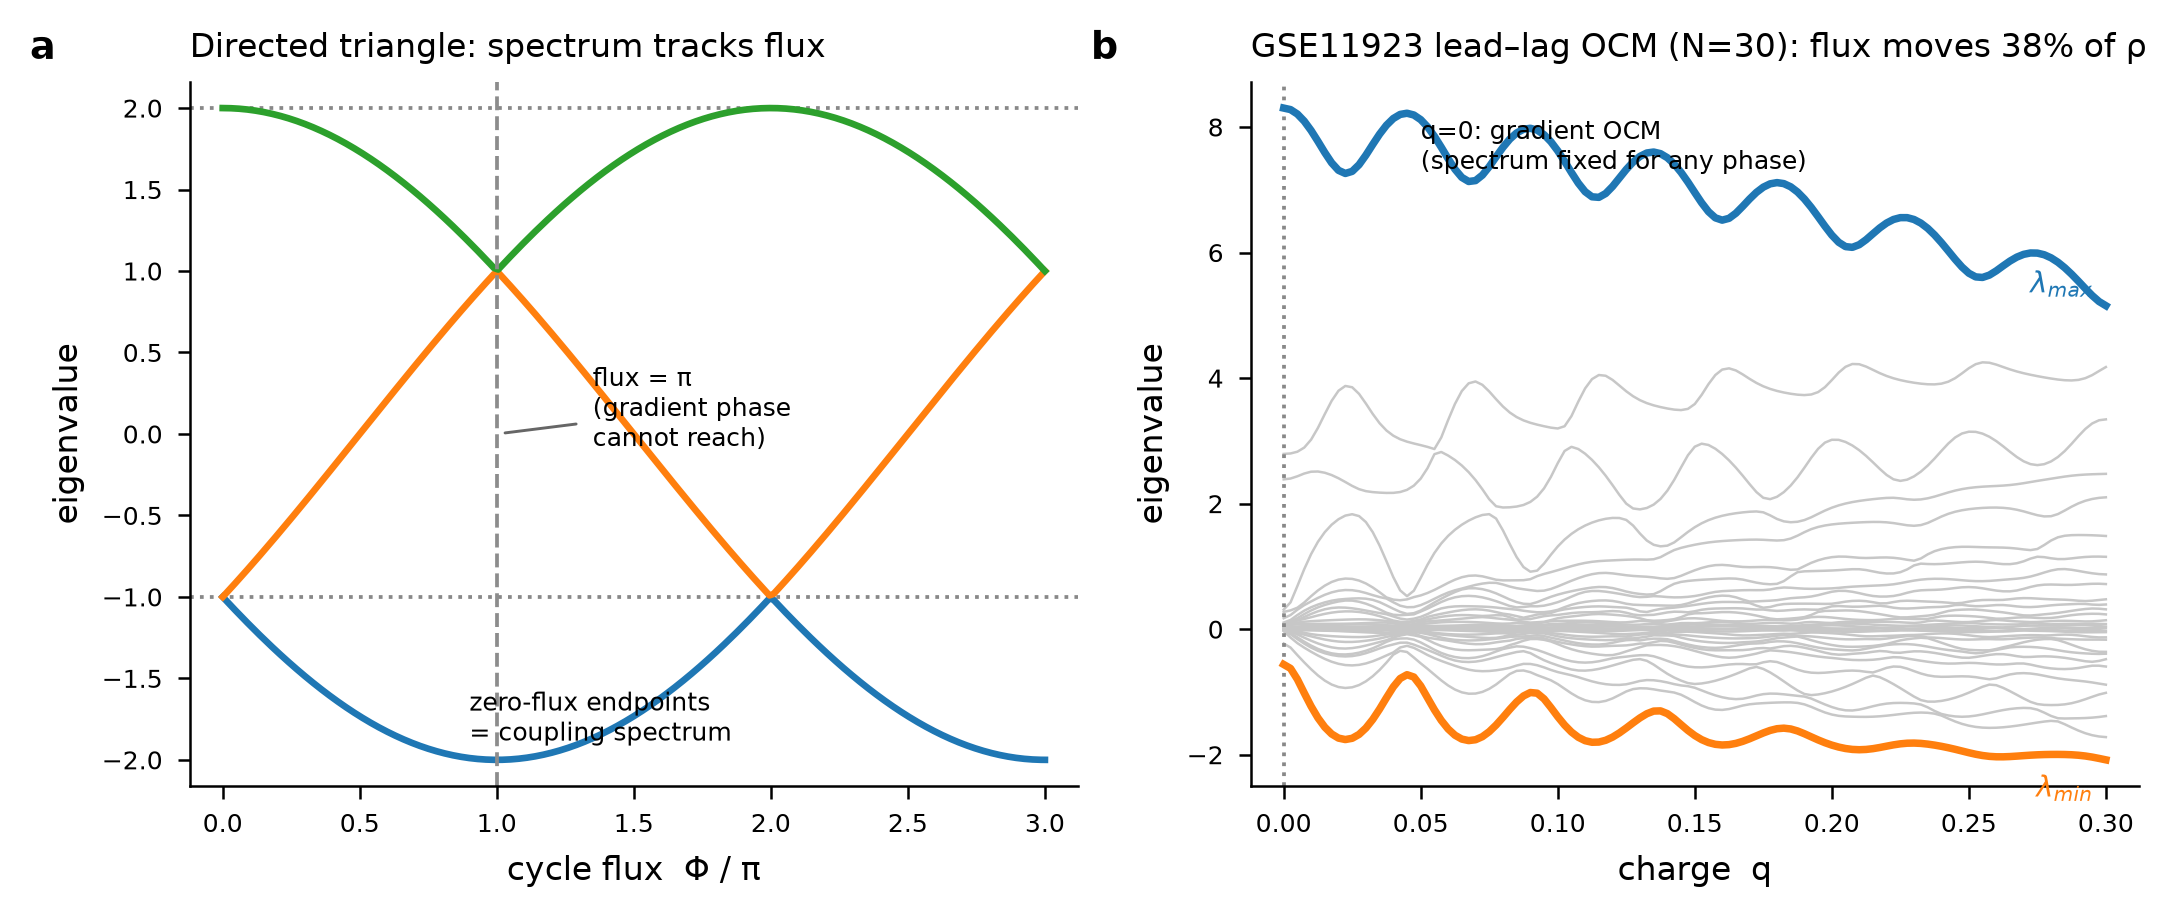
\includegraphics[width=\linewidth]{flux_spectrum_dependence.png}
  \caption{\textbf{A non-zero cycle flux makes the phase do topological work.}
  \textbf{(a)} Eigenvalues of the magnetic \OCM{} on a directed triangle as a
  function of the loop flux $\Phi/\pi$. At zero flux (dotted lines) the spectrum
  is that of the unsigned coupling, $\{-1,-1,2\}$; at $\Phi=\pi$ it becomes
  $\{-2,1,1\}$, unreachable by any gradient phase (which is isospectral with the
  real coupling for every vertex phase). \textbf{(b)} The 30 eigenvalues of the
  lead--lag magnetic \OCM{} on the GSE11923 circadian time-course versus the
  charge $q$. At $q=0$ the operator equals the amplitude-weighted real coupling;
  as $q$ grows the leading ($\lambda_{\max}$) and smallest ($\lambda_{\min}$)
  eigenvalues drift by up to $38\%$ of the spectral radius, whereas the
  gradient \OCM{} spectrum is flux-independent. The operator is Hermitian to
  machine precision throughout.}
  \label{fig:flux}
\end{figure}


\subsection{Omics harmonics}
\label{sec:theory-harmonics}

Diagonalising the \OCM,
\begin{equation}
  H\,\phi_n \;=\; \lambda_n \phi_n,\qquad
  \lambda_1\ge\lambda_2\ge\cdots\ge\lambda_N \in\mathbb{R},
  \label{eq:harmonics}
\end{equation}
yields the \emph{omics harmonics} $\{\phi_n\}$: an orthonormal basis of
collective modes of the molecular network. $\phi_1$ is the dominant mode; the
rank-$k$ truncation $H_k = \sum_{n\le k}\lambda_n\phi_n\phi_n^{\dagger}$ is the
best Hermitian rank-$k$ approximation of $H$ in Frobenius norm, the same
low-rank-denoising logic that motivates the eigengene decomposition of
\citet{alter2000svd}. The normalised spectral energy
$p_n = |\lambda_n|/\sum_k|\lambda_k|$ is the weight of mode $n$ and defines the
indicators below.

\subsection{Spectral indicators}
\label{sec:theory-indicators}

From $\{\lambda_n,\phi_n\}$ and the phasor field we compute a compact panel:
\begin{align}
  \Hspec &= -\tfrac{1}{\log N}\textstyle\sum_n p_n\log p_n \in[0,1]
    &&\text{(spectral entropy)},\\
  \Delta_F &= \lambda_1-\lambda_2 &&\text{(leading spectral gap)},\\
  \PR &= \big(\textstyle\sum_n p_n\big)^2 \big/ \textstyle\sum_n p_n^2
    &&\text{(participation ratio)},\\
  L_1 &= \textstyle\sum_i |\phi_{1,i}|^4 &&\text{(mode localisation, IPR)}.
\end{align}
Low $\Hspec$ with a large $\Delta_F$ indicates a single dominant collective mode
(coordinated regulation); high $\Hspec$ with a small $\Delta_F$ indicates a
spectrum fragmented over many competing modes. The participation ratio is the
effective number of active harmonics, and the inverse participation ratio $L_1$
measures whether the dominant mode is delocalised over the network or localised
on a few features. We additionally report the algebraic connectivity of the
coupling graph (the second-smallest eigenvalue of its Laplacian), a
$\psi$-independent property of $C$ retained for reference.

\subsection{The Compartment Coupling Matrix}
\label{sec:theory-ost}

To obtain a fixed, physiologically interpretable readout, features are
partitioned into five biological compartments $G_a$, indexed by $a\in\{$core
clock, redox, energy, signalling, biosynthesis$\}$, by marker membership
(\cref{sec:methods}); unassigned features fall back to the compartment of their
dominant harmonic. The \emph{Compartment Coupling Matrix} is the compartment contraction
of the \OCM,
\begin{equation}
  M_{ab} \;=\; \frac{1}{\sqrt{N_a N_b}}
    \sum_{i\in G_a}\sum_{j\in G_b} H_{ij},
  \qquad M = M^{\dagger},
  \label{eq:ost}
\end{equation}
a $5\times5$ Hermitian summary of intra- and inter-compartment coupling
(the $\sqrt{N_aN_b}$ normalisation removes compartment-size bias). Its positive
semi-definite covariance form $G = M^{\dagger}M \succeq 0$ yields two derived
readouts: the \emph{compartment spectral weights} $\pi_a$ (the normalised diagonal
energy of $G$), which rank compartment dominance, and the coherence scalar
$\kappa = w_1/\sum_a w_a \in[0,1]$ (with $w_a$ the eigenvalues of $G$), which
measures how concentrated the total inter-compartment coupling is in a single
collective mode. Reducing a network to a few functional-module coordinates in this
way parallels modularity- and community-based coarse-grainings of biological
networks \citep{newman2006modularity, barabasi2011network}. We introduce the \CCM{}
and the state classes (below) as \emph{candidate} readouts and test them against
external annotation in \cref{sec:enrich}; that test does not support a mechanistic
reading, and we accordingly treat this layer as a descriptive summary rather than
a validated classifier.

\subsection{Spectral state classes and the state record}
\label{sec:theory-taxonomy}

Seven spectral state classes can be assigned from the indicator
panel $(R,\Hspec,\Delta_F,\kappa)$ by ordered threshold rules
(\cref{tab:taxonomy}). We present these classes as a convenient discretisation of
the indicator space, \emph{not} as biologically validated states: the thresholds
are hand-set, and \cref{sec:enrich} finds the compartment layer they rest on is
not anchored to external annotation. The complete spectral state of a slice ---
indicators, eigenvalues, \CCM, compartment weights, and consistency residuals ---
is serialised into a portable JSON \emph{state record}, so a sample or time point
is summarised by one machine-readable object suitable for cohort-scale comparison.

\begin{table}[htbp]
\centering
\caption{\textbf{Seven spectral state classes.} Rules are
evaluated top to bottom, first match wins. Thresholds
$R_{hi}{=}0.7$, $R_{lo}{=}0.4$, $H_{hi}{=}0.7$, $H_{lo}{=}0.4$.}
\label{tab:taxonomy}
\small
\begin{ruledtabular}
\begin{tabular}{lll}
Class & Label & Condition \\
\colrule
III & Hyper-coupled          & $R\ge R_{hi}$, $\kappa\ge0.6$ \\
I   & Healthy-synchronised   & $R\ge R_{hi}$, $\Hspec\le H_{lo}$ \\
IV  & Desynchronised         & $R<R_{lo}$, $\Hspec\ge H_{hi}$ \\
V   & Fragmented             & $\Hspec\ge H_{hi}$, $\kappa\le0.3$ \\
VI  & Compartment-imbalanced & $\max_a\pi_a\ge0.5$ \\
II  & Balanced-modular       & $R_{lo}\le R<R_{hi}$, $H_{lo}<\Hspec<H_{hi}$ \\
VII & Transitional           & otherwise \\
\end{tabular}
\end{ruledtabular}
\end{table}

\subsection{Consistency suite}
\label{sec:theory-consistency}

Because the pipeline is a chain of linear-algebraic constructions, each stage
admits an exact invariant, and every run closes by checking all of them, each
returning a numerical residual: Hermiticity $\lVert H-H^{\dagger}\rVert$, real
spectrum $\max_n|\Im\lambda_n|$, eigenvector orthonormality
$\lVert\Phi^{\dagger}\Phi-I\rVert$, \CCM{} Hermiticity, positive
semi-definiteness of $G$ (least eigenvalue $\ge0$), gauge invariance (spectrum
unchanged under a random global $\alpha$), and spectral completeness
$|\operatorname{tr}H-\sum_n\lambda_n|$ evaluated over the full spectrum. These
are correctness guarantees on the implementation, not empirical claims about the
biology; they are satisfied to machine precision on real data
(\cref{sec:results}).

\subsection{Quantum-simulable correspondence}
\label{sec:theory-quantum}

Each elementary phasor operation has an exact single- or two-qubit gate analog:
a phase shift $\theta\to\theta+\delta$ corresponds to a $R_z(\delta)$ rotation,
pairwise phase coupling to a controlled-\textsc{not}, and the harmonic
(discrete-Fourier) basis change to the quantum Fourier transform
\citep{nielsen2010quantum}. This correspondence is provided for completeness and
as a route to executing the \OCM{} spectral step on quantum hardware for
networks too large for classical diagonalisation; it is not required by the
classical pipeline, and no claim is made of physical quantum computation in
cells.

% ================================================================
\section{Methods}
\label{sec:methods}

\subsection{Software}

Spectral-Omics is an installable Python package, \texttt{spectralomics}, built
only on the scientific-Python stack (NumPy, SciPy, pandas, matplotlib) with
optional data loaders (GEOparse, scanpy). Its modules mirror the pipeline:
\texttt{connectome} (phasor encoding, \OCM, harmonics), \texttt{omics}
(indicators, \CCM, compartment weights, state classes, state record, consistency, markers),
\texttt{viz} (figures), and a \texttt{quantum} module exhibiting the gate
correspondence of \cref{sec:theory-quantum}. A \texttt{SpectralOmicsPipeline}
wrapper chains the full sequence, estimating the coupling once and running each
sample slice through \crefrange{eq:ocm}{eq:ost}. All eigendecompositions use the
Hermitian solver \texttt{numpy.linalg.eigh}, which guarantees a real spectrum and
an orthonormal eigenbasis up to floating-point error. A suite of 40 unit tests
locks in the invariants of \cref{sec:theory-consistency}.

\subsection{Coupling estimation}

The default coupling is $c_{ij}=|\rho_{ij}|$, the absolute Pearson correlation of
the $\log(1+x)$ feature profiles across all samples, with $c_{ii}$ set to a
fixed self-affinity. A single global coupling is used for all slices so that
differences between samples are attributable to the phasor field rather than to a
re-estimated graph; the soft-threshold and prior-adjacency variants are exposed
for studies where a scale-free topology or a curated network is preferred
\citep{langfelder2008wgcna, barabasi2011network}. The coupling enters only
through \cref{eq:ocm}, so the harmonic structure is a property of the phasor
field on a fixed graph.

\subsection{Compartment assignment}

The five \CCM{} compartments are populated from a curated marker list carrying
both mouse and human symbols and matched case-insensitively: core-clock
transcription--translation-feedback-loop genes for the clock compartment;
peroxiredoxins, glutathione-axis and Nrf2-axis genes for redox; oxidative
phosphorylation, glycolysis and AMPK genes for energy; MAPK/PI3K and
immediate-early genes for signalling; and lipogenic, sterol and translation genes
for biosynthesis. Probes are mapped to symbols through the platform annotation of
each dataset. Features without a marker are assigned to the compartment of their
dominant omics harmonic, so every feature contributes to exactly one compartment.

\subsection{Datasets}

Both datasets are public and downloaded from the NCBI Gene Expression Omnibus
\citep{edgar2002geo} at run time (\cref{tab:data}). \textbf{GSE10072} is a
lung-adenocarcinoma cohort on the Affymetrix HG-U133A platform: 58 tumours and 49
adjacent-normal samples, with tumour/normal status read from the sample titles
\citep{landi2008gene}. \textbf{GSE11923} is a high-temporal-resolution
mouse-liver transcriptome on the Affymetrix Mouse~430\,2.0 platform: 48 samples
at one-hour spacing across circadian times CT18--CT65, spanning two full days
\citep{hughes2009harmonics}.

\begin{table}[htbp]
\centering
\caption{\textbf{Public datasets.} Both are downloaded automatically at run time;
no result depends on private or access-controlled data.}
\label{tab:data}
\small
\begin{ruledtabular}
\begin{tabular}{lll}
Accession & Shape & Role \\
\colrule
GSE10072 & $22{,}283\times107$ & lung tumour ($58$) vs.\ normal ($49$) \\
GSE11923 & $45{,}101\times48$  & mouse-liver circadian, 48 hourly points \\
\end{tabular}
\end{ruledtabular}
\end{table}

\subsection{Feature selection}

For the cancer analysis we retain the 200 most-variable probes and force in all
marker probes, giving $N=364$ features ($164$ marker-mapped). For the circadian
analysis we apply a \emph{rhythmicity gate}: each probe's $\log(1+x)$ profile is
regressed on $\{\cos\omega t,\sin\omega t,1\}$ at $\omega=2\pi/24\,\mathrm{h}$,
and the 300 probes with the highest coefficient of determination are kept
together with the clock markers, giving $N=526$ features ($241$ marker-mapped).
This linear-least-squares gate is a lightweight analog of the nonparametric and
periodogram-based rhythmicity tests standard in circadian genomics
\citep{hughes2010jtk, vanderplas2018lombscargle, cornelissen2014cosinor} and
concentrates the analysis on genes that actually oscillate. In both analyses the
leading 20 harmonics are retained for the indicator panel, while the consistency
check for spectral completeness uses the full spectrum.

\subsection{Circadian quantification}

Each spectral-indicator time series $y(t)$ is fit to a $24$-hour cosinor
$y \approx A\cos\omega t + B\sin\omega t + c$
\citep{cornelissen2014cosinor}, and we report the fraction of variance explained
$R^2$, the amplitude $\sqrt{A^2+B^2}$, and the acrophase. Group contrasts in the
cancer analysis are summarised by per-group means of $R$, $\Hspec$, and
$\Delta_F$, with the two tissue classes never used during encoding or
decomposition.

% ================================================================
\section{Results}
\label{sec:results}

\begin{figure}[htbp]
\centering
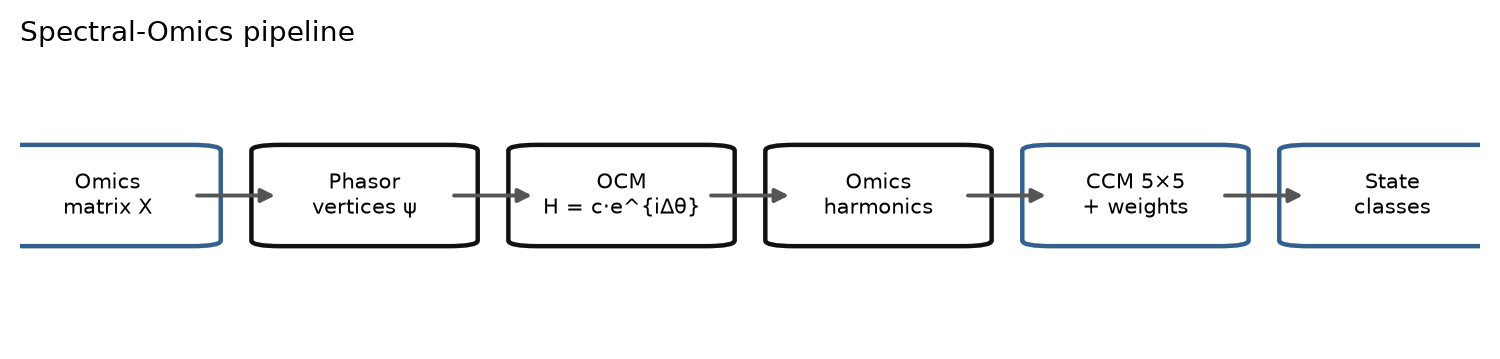
\includegraphics[width=\linewidth]{workflow.png}
\caption{\textbf{The Spectral-Omics pipeline.} An omics matrix is encoded as
phasor vertices, assembled into the Hermitian Omics Connectome Matrix,
diagonalised into omics harmonics, and read out through the $5\times5$
Compartment Coupling Matrix, the compartment spectral weights, and the seven
spectral state classes; every run closes with the algebraic consistency suite.}
\label{fig:workflow}
\end{figure}

\subsection{The construction is internally consistent}
\label{sec:res-consistency}

On both datasets all seven checks of \cref{sec:theory-consistency} pass at
machine precision: Hermiticity and \CCM{} Hermiticity are exact, the spectrum is
real, eigenvector orthonormality and gauge invariance hold to $\sim10^{-14}$, the
covariance form is positive semi-definite, and spectral completeness closes to
$\sim10^{-13}$. The gauge-invariance residual confirms empirically that a random
global phase shift leaves the \OCM{} spectrum unchanged, as required by
\cref{sec:theory-ocm}. These are correctness guarantees for the implementation;
the biological content is in the sections that follow.

\subsection{Cancer tumour/normal benchmark}
\label{sec:res-cancer-bench}

We tested whether the phasor spectral-indicator features carry discriminative
power beyond standard baselines, and specifically whether the \emph{phase}
component contributes, on lung adenocarcinoma versus adjacent normal tissue
(GSE10072; 58 tumour, 49 normal; 364 features = top-200 variable probes plus
164 compartment-marker probes). Five feature sets were compared under identical
$\ell_2$-regularised logistic regression with $5\times10$ repeated stratified
cross-validation: the phasor spectral indicators (spectral entropy, Fiedler
gap, participation ratio, mode localisation, Kuramoto $R$); a \emph{phase-free}
ablation of the same panel with $\theta_i\!=\!0$ (so the OCM reduces to the
real amplitude-only form $H^0_{ij}=c_{ij}r_ir_j$); the top-10 principal-component
scores of the $\log_{1+}$ expression matrix; and 10 WGCNA-style module
eigengenes. All feature extraction (phasor phase/amplitude standardisation,
the coupling correlation matrix, PCA, and the WGCNA modules) was fit inside the
training folds only, so the held-out AUROC is leakage-free. Confidence intervals
are 2000-sample bootstraps of the pooled out-of-fold predictions.

Every feature set separates the two classes near the ceiling of the metric
(Fig.~\ref{fig:bench}a): phase-free AUROC $=0.997$ (95\% CI $0.989$--$1.000$), phasor
$=0.998$ ($0.993$--$1.000$), PCA $=0.999$ ($0.996$--$1.000$), and WGCNA eigengenes $=0.998$
($0.990$--$1.000$); accuracies were $0.972$--$0.991$. The decisive test---phasor versus its
own phase-free ablation---shows \textbf{no benefit from the phase}: the mean
per-repeat AUROC difference is $+0.001$ (Wilcoxon signed-rank $p=0.80$, Cohen's
$d_z=0.12$ over 10 repeats). Because the full-sample comparison sits against the
metric ceiling, we repeated the phasor-versus-phase-free contrast at reduced
training sizes ($n_{\mathrm{train}}=16,24,40$; 20 resamples each) to expose any
difference off-ceiling (Fig.~\ref{fig:bench}b). The two remained statistically
indistinguishable at every size (paired Wilcoxon $p=0.26$, $0.27$, $0.055$
respectively; at $n_{\mathrm{train}}=16$ the phase-free variant was in fact
marginally higher). On this
tumour/normal contrast the phasor construction matches strong linear baselines,
but the phase factor $e^{i(\theta_i-\theta_j)}$ adds no measurable
discriminative power.

\begin{table}[t]
\centering
\caption{GSE10072 tumour vs.\ normal: held-out AUROC (pooled out-of-fold, with
bootstrap 95\% CI), accuracy, and $F_1$ under $5\times10$ repeated stratified
CV. The phasor and its phase-free ablation are statistically indistinguishable.}
\label{tab:bench}
\begin{tabular}{lcccc}
\hline
Feature set & AUROC & 95\% CI & Accuracy & $F_1$ \\
\hline
Phase-free (amplitude only) & 0.997 & 0.989--1.000 & 0.972 & 0.974 \\
Phasor (full, with phase)   & 0.998 & 0.993--1.000 & 0.972 & 0.974 \\
PCA (top-10)                & 0.999 & 0.996--1.000 & 0.972 & 0.974 \\
WGCNA eigengenes            & 0.998 & 0.990--1.000 & 0.991 & 0.991 \\
\hline
\end{tabular}
\end{table}

\begin{figure}[t]
\centering
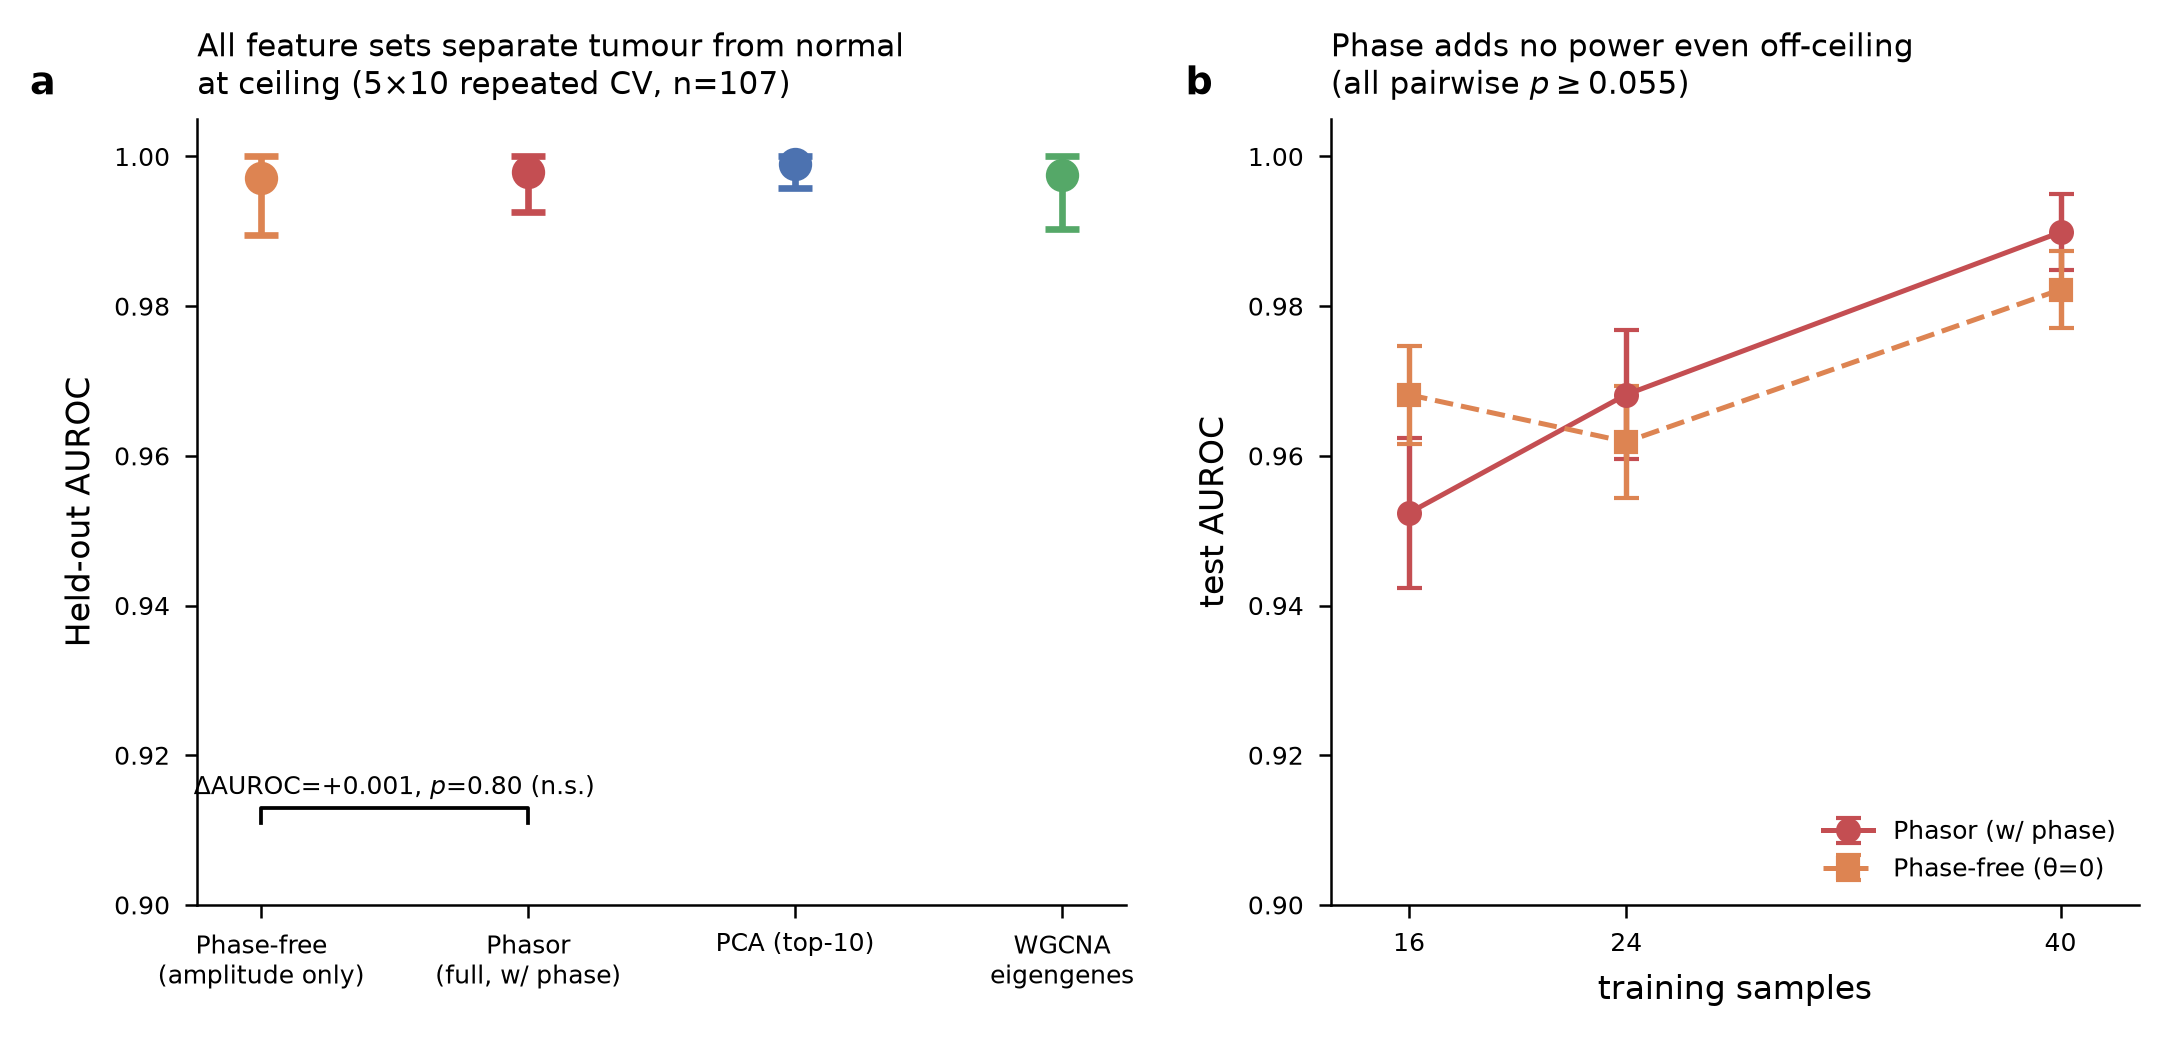
\includegraphics[width=\linewidth]{bench_auroc_comparison.png}
\caption{\textbf{Phasor spectral features match baselines but the phase adds no
discriminative power (GSE10072, 58 tumour / 49 normal).}
(a) Held-out AUROC (pooled out-of-fold point, bootstrap 95\% CI whiskers) under
$5\times10$ repeated stratified CV with leakage-safe feature extraction. All
four feature sets---phase-free amplitude-only indicators, the full phasor
indicators, top-10 PCA, and 10 WGCNA module eigengenes---sit at the ceiling of
the metric; the phasor-vs.\ phase-free increment is not significant.
(b) Learning-curve control at small training sizes, where AUROC is below
ceiling: the phasor (with phase) and phase-free ($\theta=0$) variants remain
statistically indistinguishable at every size (paired Wilcoxon $p\geq0.055$;
error bars are $\pm$SEM over resamples).}
\label{fig:bench}
\end{figure}


\FloatBarrier

\subsection{Descriptive spectral structure of the tumour/normal contrast}
\label{sec:res-cancer-descriptive}

Although the phase adds no discriminative power (\cref{sec:res-cancer-bench}), the
spectral indicators remain an interpretable description of transcriptional
coordination. Adjacent-normal tissue has lower spectral entropy
($\Hspec\approx0.61$) and a larger leading gap ($\Delta_F\approx55$) than tumour
tissue ($\Hspec\approx0.75$, $\Delta_F\approx28$): the normal network is dominated
by a single coherent collective mode, whereas the tumour spectrum is more
fragmented (\cref{fig:cancer-sep}). This is consistent with the eigengene view
that a few dominant modes capture coherent regulatory programmes
\citep{alter2000svd}; we present it as description, not as a phasor-specific
classifier. The compartment-level readout of a representative tumour
(\cref{fig:cancer-ost-oma}) shows the amplitude-weighted \CCM{} $|M_{ab}|$ and the
compartment weights; we return in \cref{sec:enrich} to whether this compartment
layer is anchored to external annotation.

\begin{figure}[htbp]
\centering
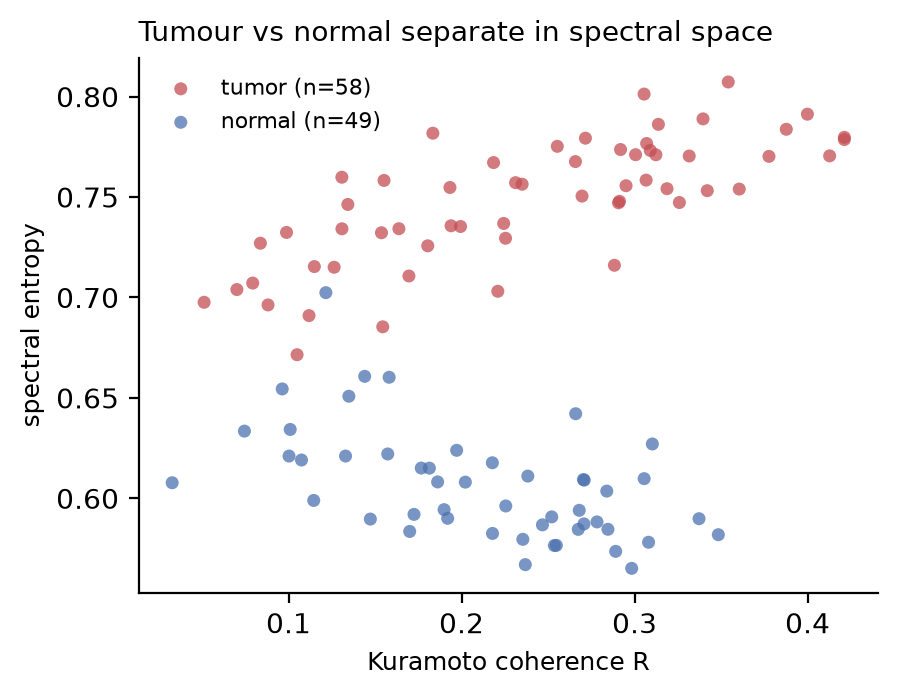
\includegraphics[width=0.82\linewidth]{cancer_indicator_separation.png}
\caption{\textbf{Descriptive spectral structure of lung tumour and normal
tissue.} Each point is one sample in the plane of Kuramoto coherence $R$ and
spectral entropy $\Hspec$ (tumour red, normal blue). The classes differ along
$\Hspec$ --- normal tissue is spectrally concentrated, tumours more fragmented ---
but this separation is matched by phase-free and standard baselines
(\cref{tab:bench}).}
\label{fig:cancer-sep}
\end{figure}

\begin{figure}[htbp]
\centering
\begin{subfigure}{0.49\linewidth}
  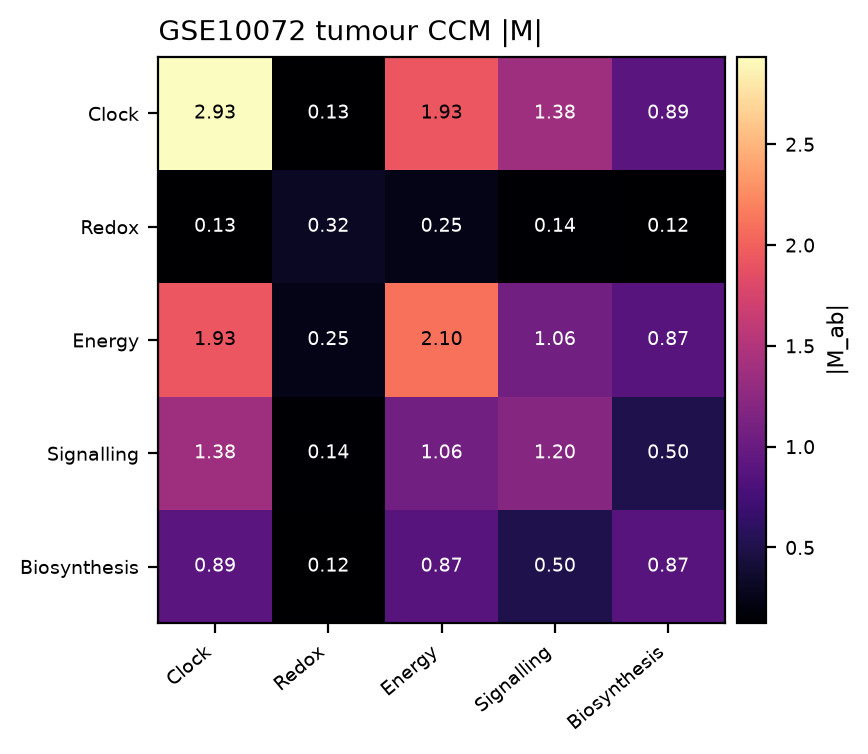
\includegraphics[width=\linewidth]{cancer_ost_heatmap.png}
  \caption{}
  \label{fig:cancer-ost}
\end{subfigure}\hfill
\begin{subfigure}{0.49\linewidth}
  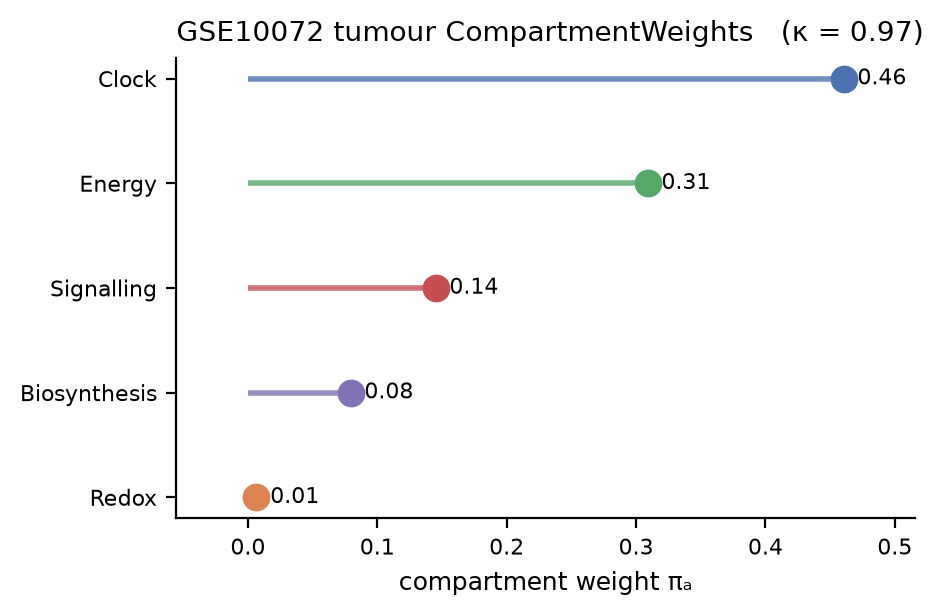
\includegraphics[width=\linewidth]{cancer_omicatome.png}
  \caption{}
  \label{fig:cancer-oma}
\end{subfigure}
\caption{\textbf{Compartment-level readout for a representative tumour
(descriptive).}
(a) Magnitude of the amplitude-weighted Compartment Coupling Matrix $|M_{ab}|$.
(b) The corresponding compartment spectral weights and coherence $\kappa$.
The biological anchoring of this layer is assessed in \cref{sec:enrich}.}
\label{fig:cancer-ost-oma}
\end{figure}

\FloatBarrier

% circ2_ : circadian phase recovery and out-of-sample validation
\subsection{The phasor recovers circadian phase out-of-sample}
\label{sec:res-circadian}

We establish three properties of the circadian analysis: that the phasor phase
recovers biological timing, that the collective spectral rhythm is not reducible
to mean expression, and that it persists under a selection protocol independent of
the tested rhythm. All three tests use the mouse liver time-course
GSE11923 \citep{hughes2009harmonics} (48 hourly samples, CT18--65).

\textbf{Phase-lag recovery.} For the twelve core-clock genes present on the array
(\textit{Nr1d1}, \textit{Nr1d2}, \textit{Dbp}, \textit{Per1/2/3}, \textit{Cry1/2},
\textit{Arntl}/Bmal1, \textit{Nfil3}, \textit{Tef}, \textit{Hlf}) we recovered each
gene's circadian acrophase from the Spectral-Omics phasor phase $\theta$ and compared
it to a direct 24\,h cosinor fit and to the established physiological peak order. The
recovered acrophases are essentially identical to the cosinor acrophases
(circular correlation $r_{\mathrm{circ}}=0.997$) and reproduce the known
ordering---\textit{Nr1d1}/\textit{Dbp} in the early-to-mid subjective day,
\textit{Per} genes near CT12, and \textit{Arntl}/Bmal1 in antiphase---with
$r_{\mathrm{circ}}=0.93$ against literature peak times
(Fig.~\ref{fig:circ2_phaselag}). The Bmal1--\textit{Per1} phase separation is
11.2\,h, i.e.\ the expected $\sim$12\,h antiphase between the positive and
negative limbs of the clock. The phasor encoding therefore preserves, rather than
discards, circadian phase.

\textbf{Spectral rhythm is not the mean-expression rhythm.} On the same gene set we
compared the 24\,h cosinor $R^2$ of the collective spectral indicators to that of the
simple mean log-expression (Fig.~\ref{fig:circ2_spectral}). The leading eigenvalue
$\lambda_1$ largely tracks the mean (Pearson $r=0.87$, $R^2=0.40$), so it
adds little beyond magnitude. The participation ratio, however, oscillates more
strongly than the mean ($R^2=0.68$ vs.\ $0.62$), is nearly orthogonal to
it (Pearson $r=0.21$), and peaks several hours later---structure the mean does
not carry. The spectral rhythm is thus partly, but not wholly, reducible to mean
expression.

\textbf{Out-of-sample selection.} To separate gene selection from the tested
rhythm, we
selected rhythmic genes on the first day only (CT18--41; top 200 by cosinor $R^2$) and
tested the collective spectral oscillation on the held-out second day (CT42--65). The
out-of-sample 24\,h rhythm persists strongly: $\lambda_1$ $R^2=0.73$ and Fiedler
gap $R^2=0.77$ on unseen timepoints (permutation $p=0.0005$ for $\lambda_1$,
null 95th percentile $R^2=0.26$), both exceeding the held-out mean-expression fit
($R^2=0.35$). As a rhythm-blind control, selecting the 200 highest-variance
probes yields only weak collective rhythm ($\lambda_1$ $R^2=0.16$), confirming the
signal is carried by genuinely rhythmic---not merely high-variance---genes. The
circadian claim is therefore phase-informative and holds out-of-sample.


\begin{figure}[htbp]
\centering
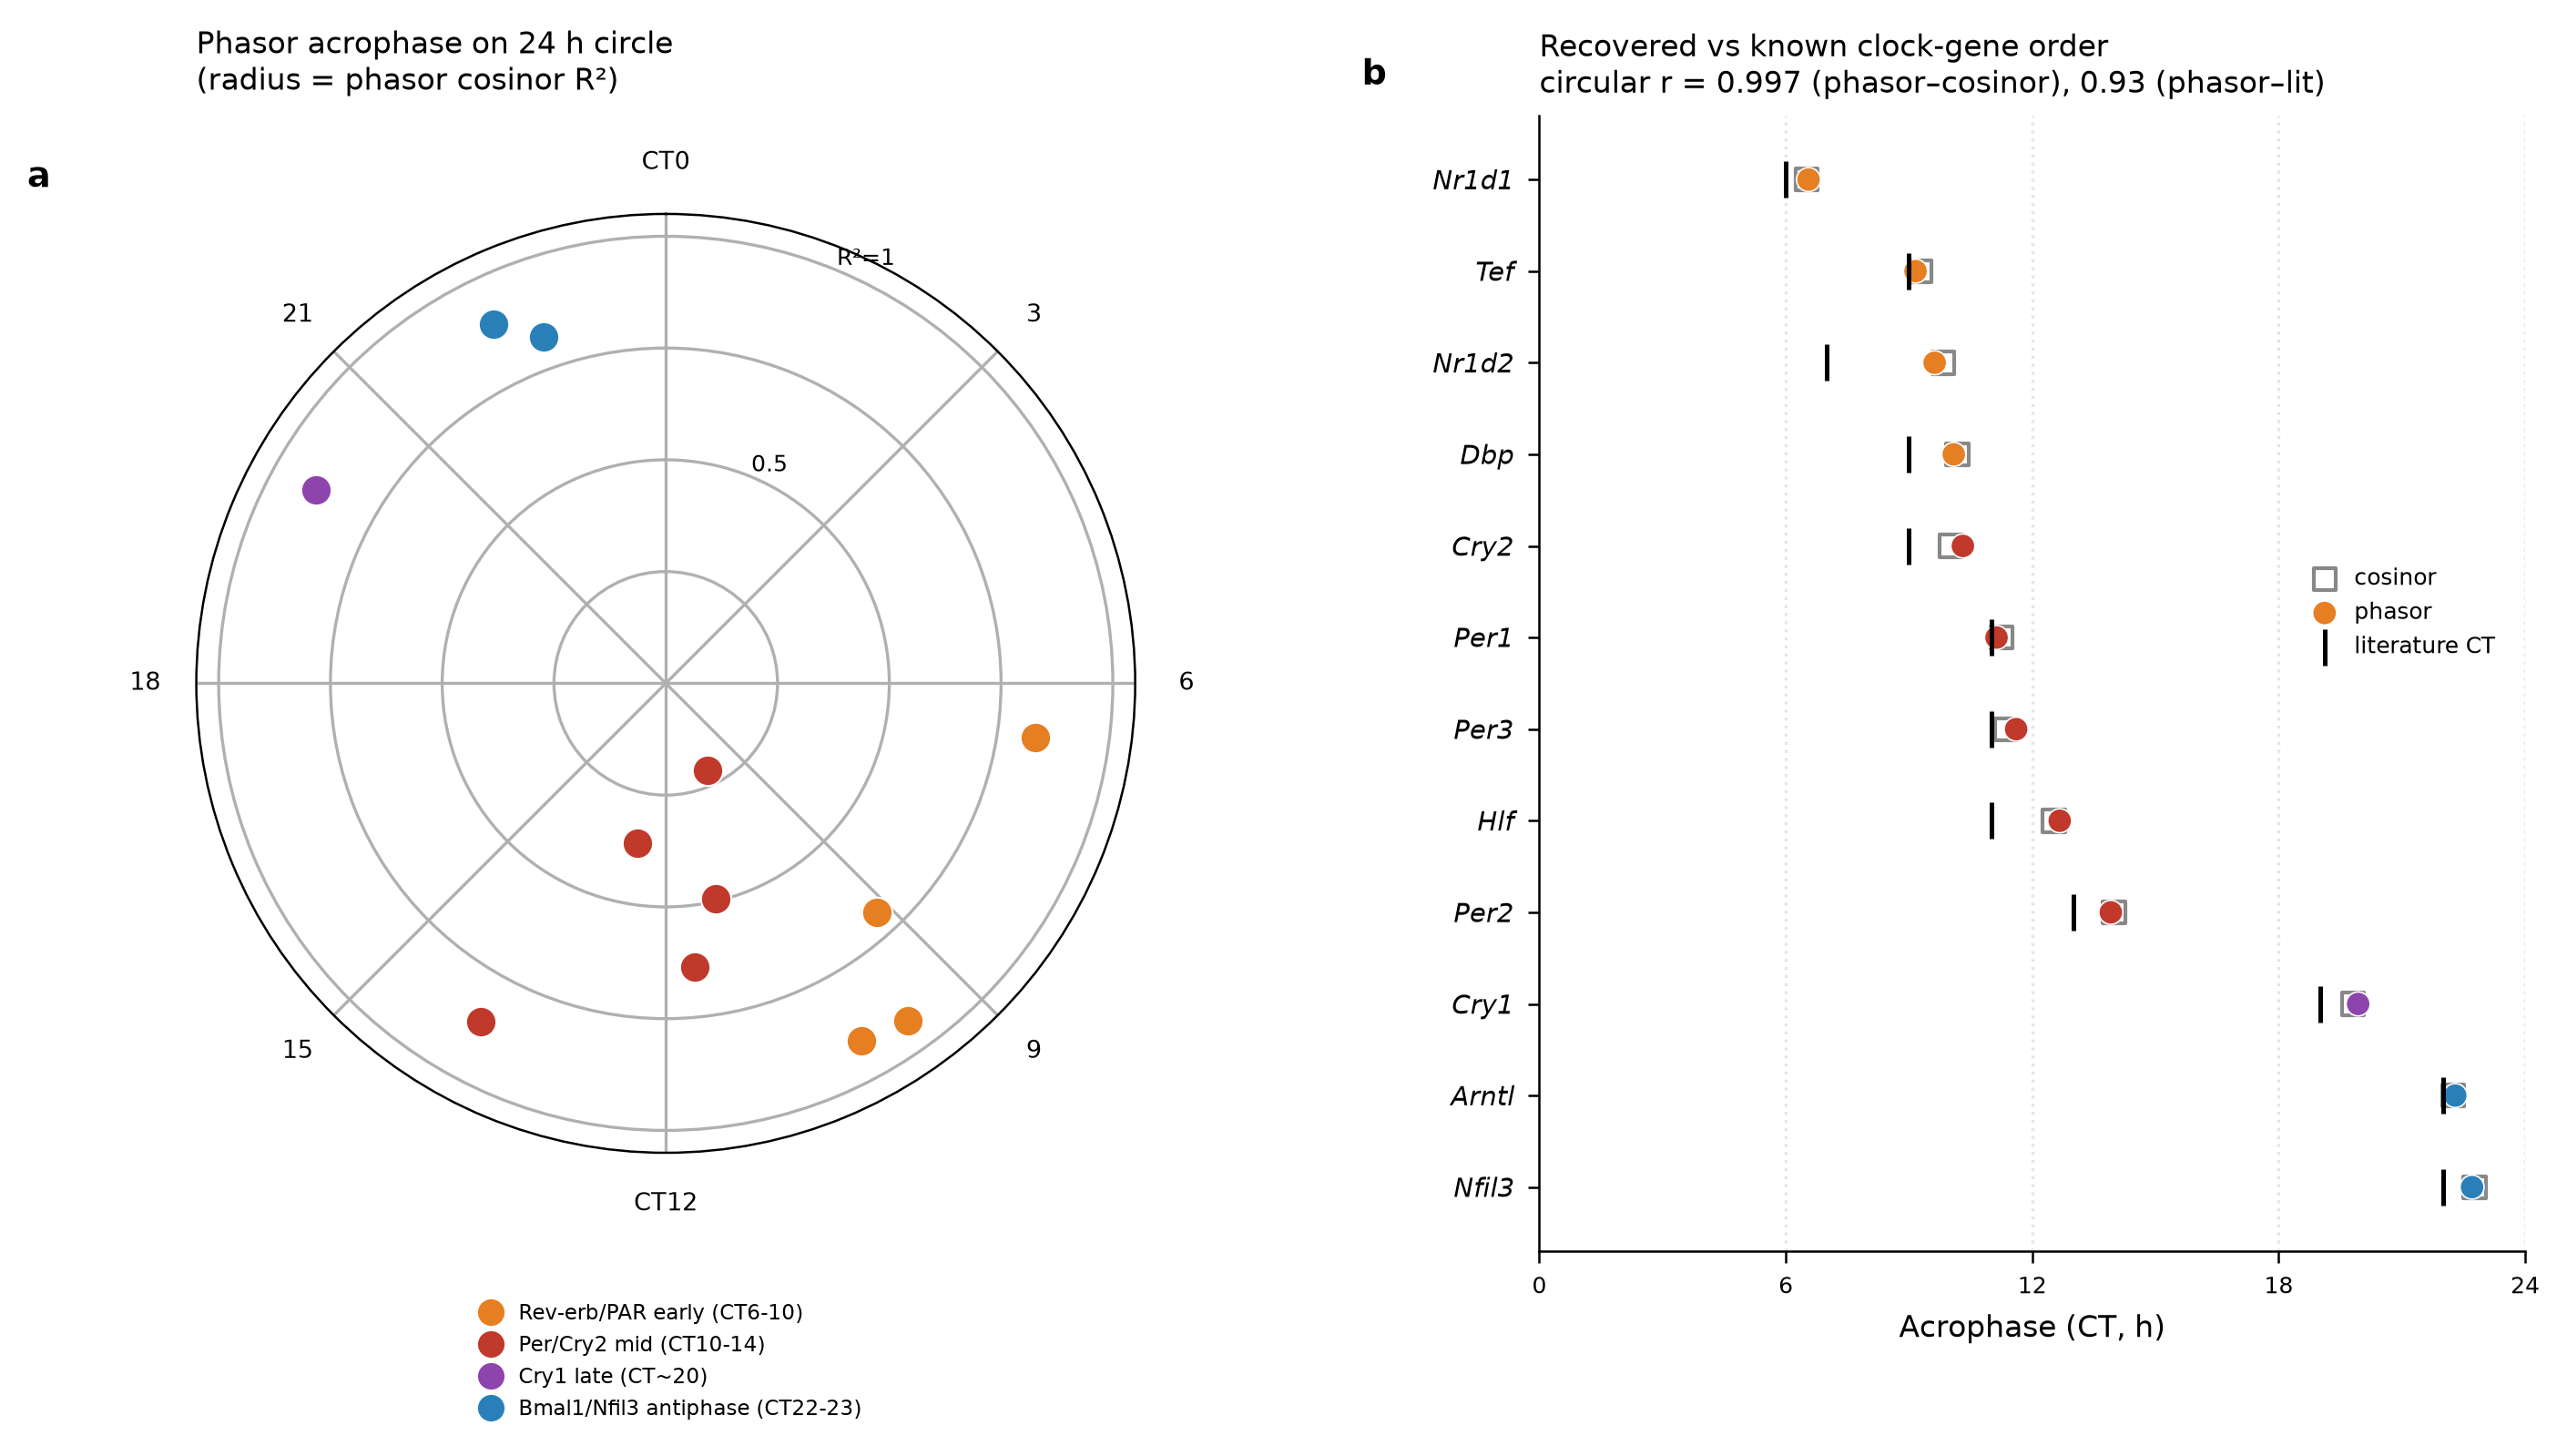
\includegraphics[width=0.9\linewidth]{circ2_phase_lag.png}
\caption{\textbf{The phasor recovers core-clock phase.} Circadian acrophase of
twelve core-clock genes recovered from the Spectral-Omics phasor phase versus a
direct $24$-hour cosinor fit (circular correlation $r_{\mathrm{circ}}=0.997$); the
known positive/negative-limb antiphase (\emph{Arntl}/Bmal1 vs.\ \emph{Per}) is
reproduced.}
\label{fig:circ2_phaselag}
\end{figure}

\begin{figure}[htbp]
\centering
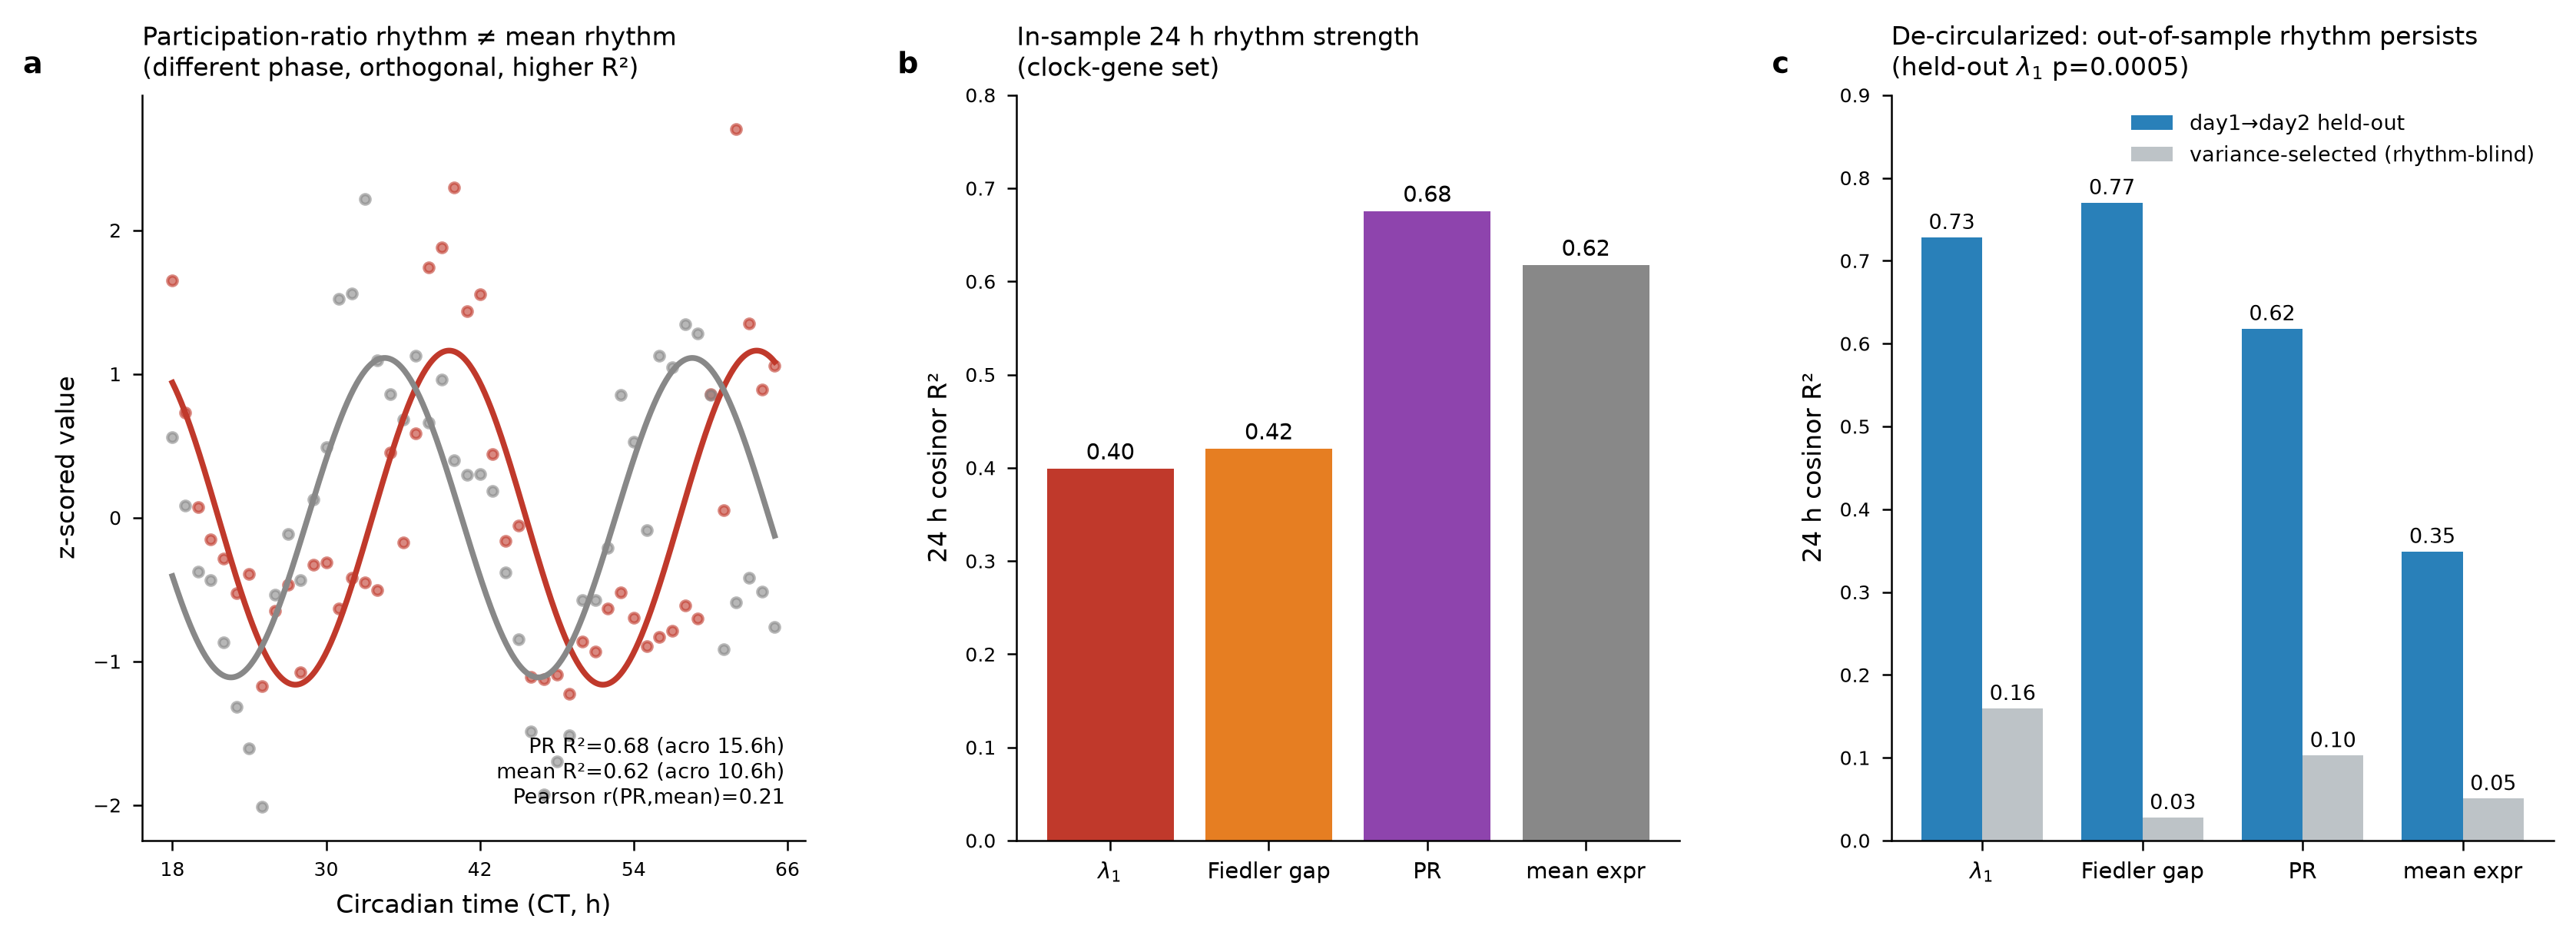
\includegraphics[width=0.9\linewidth]{circ2_spectral_vs_mean.png}
\caption{\textbf{The spectral rhythm is not merely the mean-expression rhythm.}
$24$-hour cosinor fit of the collective spectral indicators versus the mean
log-expression of the same gene set. The leading eigenvalue $\lambda_1$ largely
tracks the mean ($r=0.87$), but the participation ratio oscillates more strongly
($R^2=0.68$ vs.\ $0.62$) and is nearly orthogonal to it ($r=0.21$).}
\label{fig:circ2_spectral}
\end{figure}

\begin{figure}[htbp]
\centering
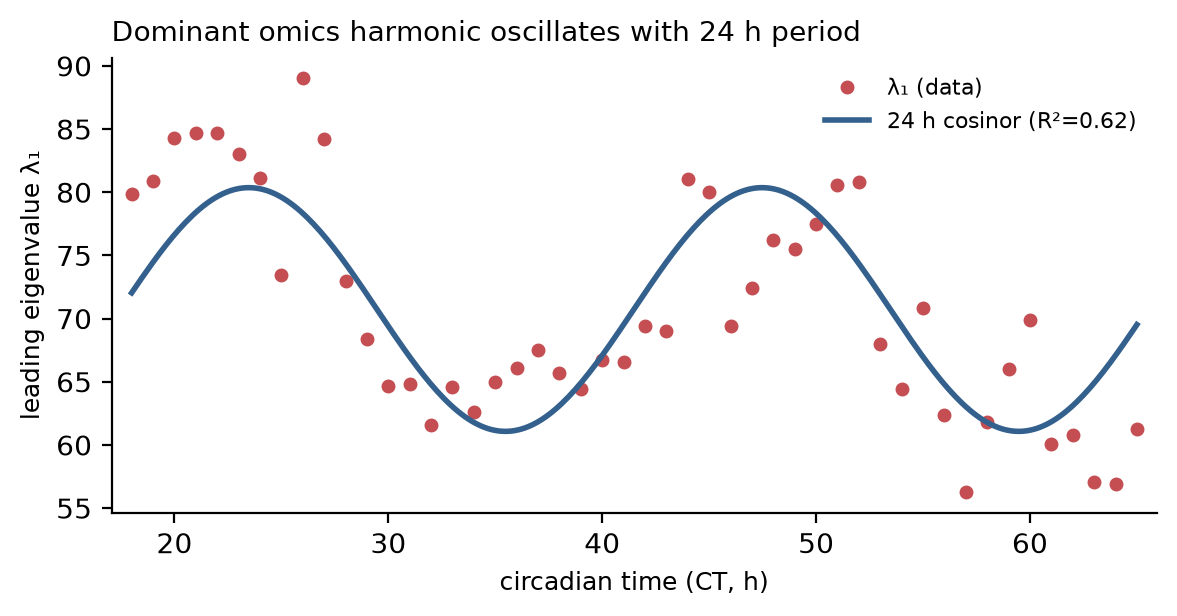
\includegraphics[width=0.9\linewidth]{circadian_leading_harmonic_fit.png}
\caption{\textbf{The leading omics harmonic oscillates with the circadian clock.}
$\lambda_1$ of the liver transcriptome (points) across CT18--CT65; the solid line
is the $24$-hour cosinor fit. Two full circadian cycles are covered. Note
(\cref{fig:circ2_spectral}) that $\lambda_1$ largely mirrors mean expression; the
non-redundant collective signal is carried by the participation ratio.}
\label{fig:circ-fit}
\end{figure}

\begin{figure}[htbp]
\centering
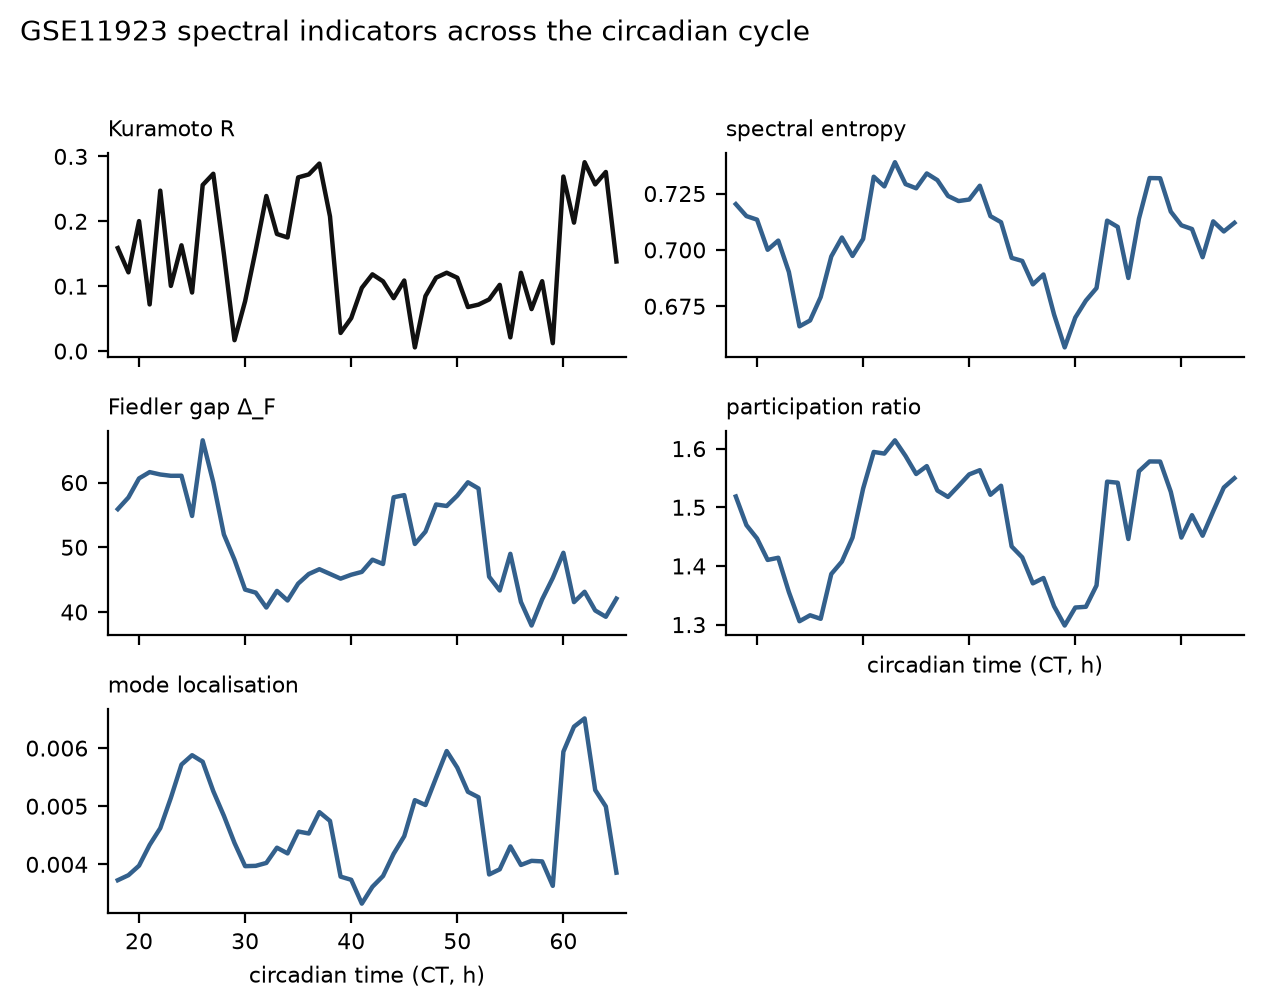
\includegraphics[width=\linewidth]{circadian_indicator_dashboard.png}
\caption{\textbf{Spectral indicators across the circadian cycle.} The Fiedler gap
and participation ratio show the strongest $24$-hour rhythm; the algebraic
connectivity, a property of the fixed coupling alone, carries no per-slice signal
and is omitted.}
\label{fig:circ-dash}
\end{figure}

\FloatBarrier

% ===== enrich_ : Module & taxonomy validation (Phase 4) =====
\subsection{Biological annotation of the leading harmonics and the compartment layer}
\label{sec:enrich}

We tested whether the leading omics harmonics correspond to coherent biological
programmes, and whether the five-compartment / seven-class layer is anchored to
ground-truth annotation. For each dataset we aggregated the per-slice loading
magnitude $\langle|\varphi_{n,i}|\rangle_s$ of the three leading harmonics and ran
hypergeometric over-representation analysis (ORA) on the top-40 loading genes against
nine hand-curated gene sets (circadian clock, cell cycle, OXPHOS/energy,
immune/inflammation, sterol/lipid biosynthesis, redox/antioxidant, ECM/adhesion,
IEG/signalling, xenobiotic metabolism; sets defined explicitly in the analysis code),
using all mapped features as the background and Benjamini--Hochberg FDR correction.
Enrichment was fully offline; no live annotation service was queried.

\paragraph{The leading harmonic $\varphi_1$ is an expression-magnitude artefact, not a
programme.} On \emph{neither} dataset did the top-loading genes of $\varphi_1$ enrich
any gene set (minimum adjusted $p = 1.00$ on GSE10072; $0.77$ on GSE11923). Across all
three leading harmonics the circadian dataset (GSE11923) produced no significant term
(minimum adjusted $p = 0.77$). The reason is mechanical: because the omics connectome
matrix is amplitude-weighted ($H_{ij}=c_{ij}\,\psi_i\psi_j^\ast$), $|\varphi_{1,i}|$
tracks mean log-expression per feature (Spearman $\rho = 0.43$ on GSE10072, $\rho =
0.42$ on GSE11923; both $p<10^{-17}$). The dominant mode therefore reports which genes
are highly expressed, not which genes co-regulate.

\paragraph{Core-clock genes do \emph{not} load preferentially on $\lambda_1$.} The
central prediction --- that in circadian data the clock module dominates the leading
harmonic --- is refuted. On GSE11923 core-clock genes load \emph{below} background on
$\varphi_1$ (one-sided Mann--Whitney for clock $>$ background $p = 0.996$, rank-biserial
$= -0.23$); the same holds on GSE10072 ($p > 0.999$, rank-biserial $= -0.40$)
(Fig.~\ref{fig:enrich_clock}). Clock genes carry moderate, not extreme, expression and
so sit in the body of the $|\varphi_1|$ distribution.

\paragraph{Sub-leading modes recover annotation-supported biology --- on the cancer
dataset only.} Once the amplitude-dominated $\varphi_1$ is set aside, coherent
programmes appear in the sub-leading harmonics of GSE10072: $\varphi_2$ enriches the
redox/antioxidant set ($k=9$, adjusted $p = 2.9\times10^{-3}$) and the circadian-clock
set (adjusted $p = 1.4\times10^{-2}$), and $\varphi_3$ enriches IEG/signalling ($k=9$,
adjusted $p = 5.1\times10^{-3}$) (Fig.~\ref{fig:enrich_ora}). Consistently, four of the
five compartment marker sets load preferentially on $\varphi_2$ in GSE10072 (Clock,
Redox, Signalling, Biosynthesis all Mann--Whitney $p<0.01$; Energy $p=0.10$). No
sub-leading harmonic reached significance on the circadian dataset, and no compartment
marker set loaded preferentially there.

\paragraph{The compartment layer is descriptive, not a validated classifier.}
The evidence does not support a mechanistic reading of the leading mode or of a
seven spectral state classes. The leading harmonic is an expression-magnitude summary; the
clock-loading prediction does not hold on the circadian dataset; and the
only annotation-supported structure is confined to sub-leading modes and
present in one of the two datasets. We therefore treat the Compartment Coupling
Matrix and the spectral state classes as a descriptive decomposition rather than a
mechanistic classifier: the sub-leading harmonics of the cancer dataset provide an
annotation-consistent decomposition, but the leading mode and the five compartments
should not be read as a ground-truth-anchored biological classifier.

\begin{figure}[t]
  \centering
  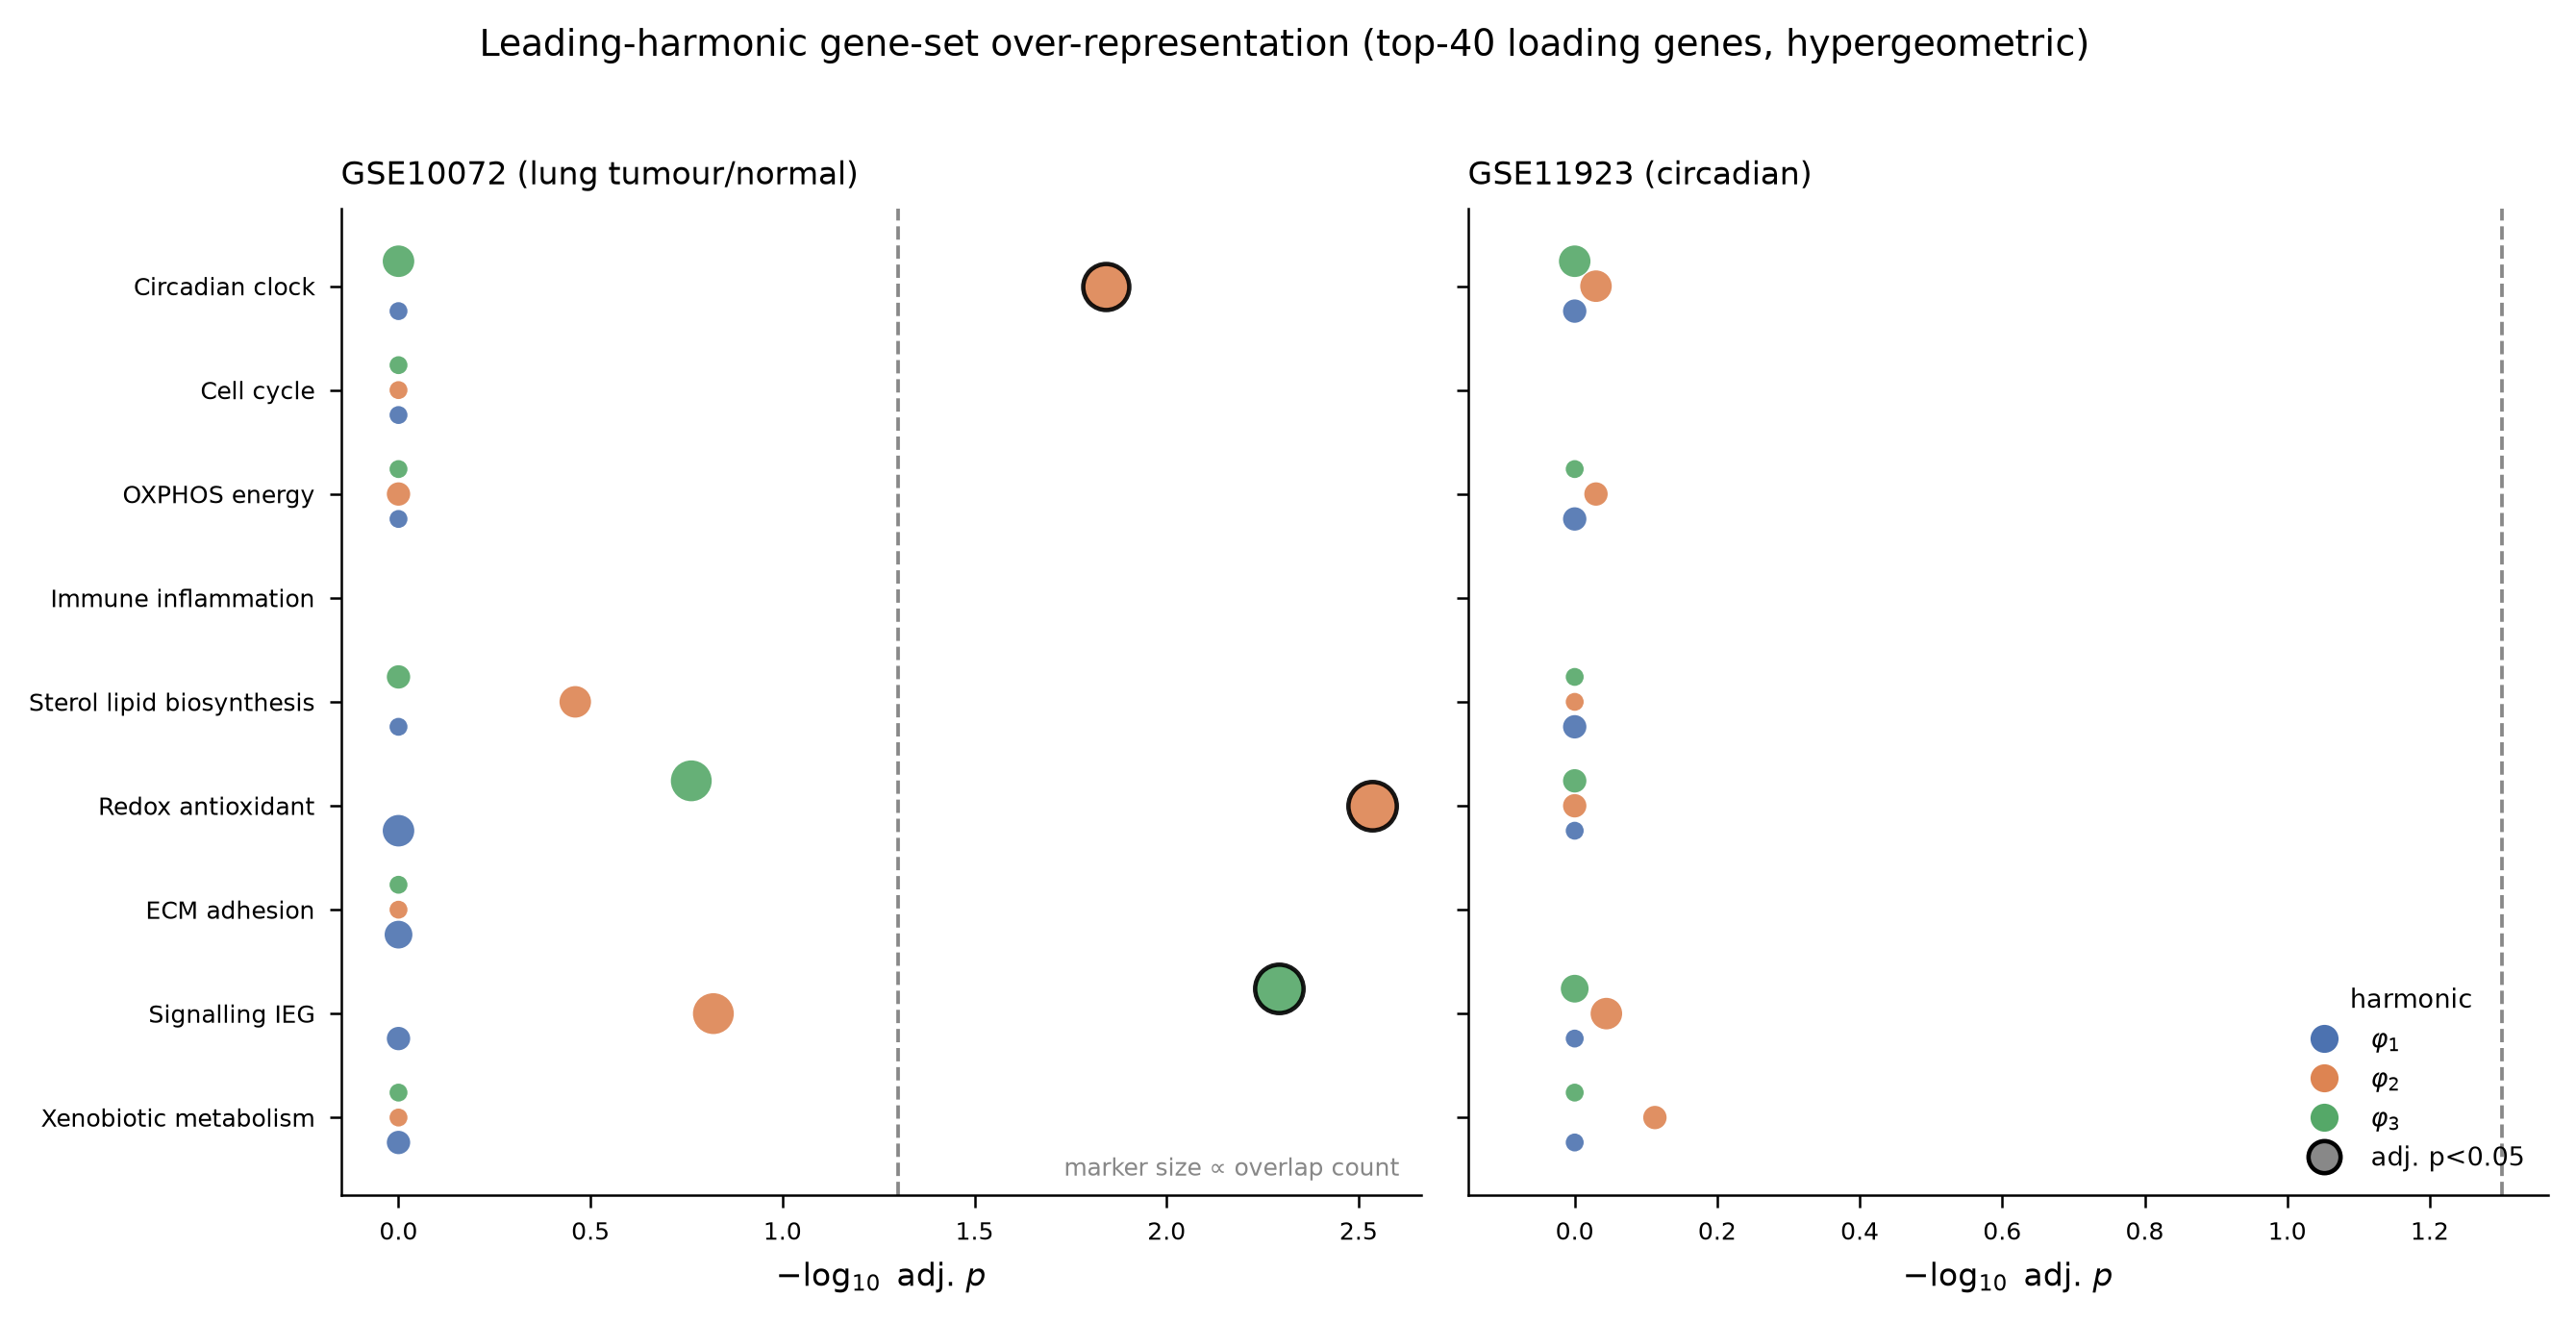
\includegraphics[width=\linewidth]{enrich_harmonic_enrichment.png}
  \caption{Hypergeometric over-representation of nine curated gene sets among the top-40
  loading genes of the three leading harmonics ($\varphi_1$ blue, $\varphi_2$ orange,
  $\varphi_3$ green), for the cancer (GSE10072, left) and circadian (GSE11923, right)
  datasets. Marker size is proportional to the overlap count; black-outlined markers are
  significant at BH-adjusted $p<0.05$ (dashed line). The leading harmonic $\varphi_1$
  enriches nothing on either dataset; significant terms appear only in the sub-leading
  modes of the cancer dataset.}
  \label{fig:enrich_ora}
\end{figure}

\begin{figure}[t]
  \centering
  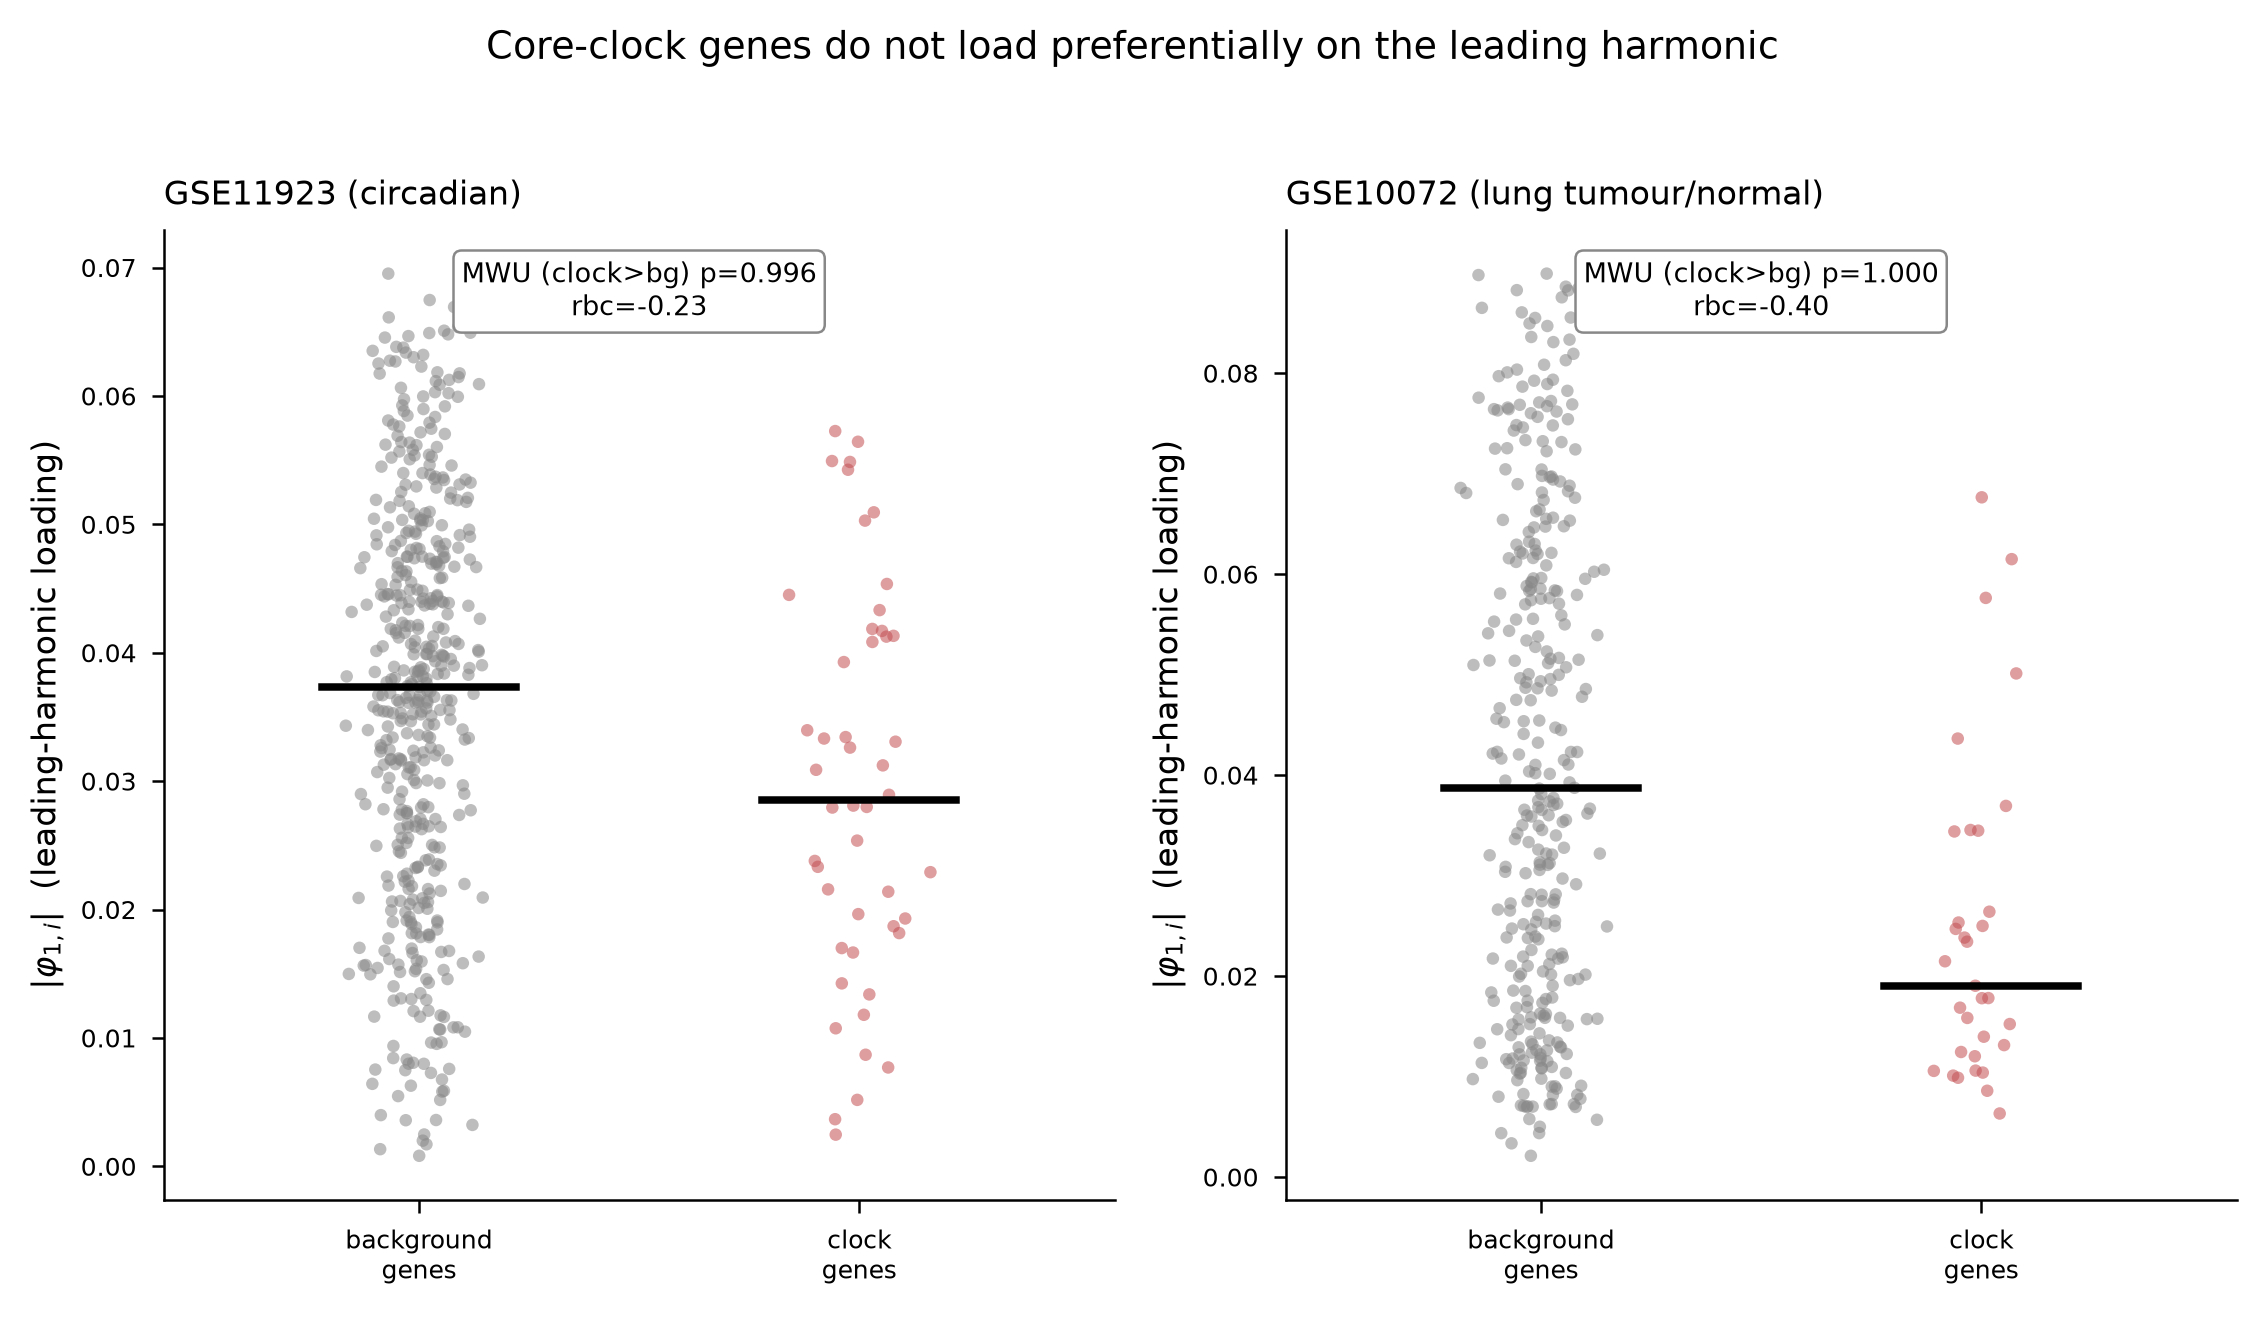
\includegraphics[width=0.85\linewidth]{enrich_clock_loading.png}
  \caption{Leading-harmonic loading $|\varphi_{1,i}|$ of core-clock genes (red) versus
  all other features (grey); black bars are group medians. In both the circadian
  (GSE11923, left) and cancer (GSE10072, right) datasets clock genes load at or below
  background, refuting the prediction that the clock module dominates $\lambda_1$
  (one-sided Mann--Whitney $p$ and rank-biserial correlation annotated).}
  \label{fig:enrich_clock}
\end{figure}


\FloatBarrier

% ================================================================
\section{Discussion and Conclusion}
\label{sec:conclusion}

We have presented Spectral-Omics, a phase-aware graph-spectral framework for
multi-omics data. Encoding molecular features as phasor vertices and building the
amplitude-weighted Hermitian Omics Connectome Matrix turns an omics matrix into a
set of real-valued collective harmonics whose spectrum is sample-specific,
gauge-invariant, and internally consistent to machine precision. Its value
depends on whether the biological question involves timing.

\paragraph{Where the phase is informative.}
For a static contrast --- lung tumour versus
normal --- the phasor spectral indicators separate the classes at the ceiling of
the metric, but so do an amplitude-only ablation, PCA, and WGCNA eigengenes, and
the phase factor $e^{i(\theta_i-\theta_j)}$ adds no measurable discriminative
power (\cref{sec:res-cancer-bench}). This follows from the construction: in a
single static snapshot the tanh phase is a deterministic monotone function of the
same abundance that sets the amplitude, so it carries little independent
information, and --- being a gradient --- it is gauge-equivalent to a phaseless
real operator (\cref{sec:flux}). The phase becomes informative when timing is the
signal. On the circadian time-course the phasor recovers core-clock acrophases
(circular correlation $0.997$ against cosinor, correct Bmal1--\emph{Per}
antiphase) and a collective rhythm that survives out-of-sample and
is distinct from --- and stronger than --- the mean-expression rhythm
(\cref{sec:res-circadian}). That rhythm lives in the relative phases of the
features, the degree of freedom a real-valued decomposition such as
SVD/PCA \citep{alter2000svd} cannot represent. In this respect Spectral-Omics is
to time-resolved gene-expression graphs what the phasor representation is to
fluorescence decays \citep{digman2008phasor, stringari2011cell}: a change of
coordinates that makes relative timing geometric, most useful when a
temporal or otherwise phase-bearing axis is present.

\paragraph{The interpretive layer.}
Because the \OCM{} is amplitude-weighted, the leading harmonic $\varphi_1$ is an
expression-magnitude summary rather than a co-regulation programme, and the
prediction that core-clock genes dominate $\varphi_1$ in circadian data does not
hold (\cref{sec:enrich}). Annotation-supported structure appears only in
sub-leading modes, and only on the cancer dataset. We therefore present the
Compartment Coupling Matrix and the spectral state classes as a descriptive
decomposition of the indicator space rather than a validated classifier.

\paragraph{Relation to existing spectral methods.}
The pipeline sits alongside a large body of spectral analysis in biology --- SVD
eigengenes \citep{alter2000svd}, co-expression modules
\citep{langfelder2008wgcna}, spectral clustering and modularity
\citep{vonluxburg2007tutorial, newman2006modularity}, connectome harmonics
\citep{atasoy2016connectome}, and diffusion maps \citep{haghverdi2015diffusion}.
It differs in using a Hermitian, complex-valued operator. The default gradient
edge-phase makes the operator gauge-equivalent to a real affinity graph
(\cref{sec:flux}), so on an undirected co-expression graph the phase is an
interpretable decoration rather than a source of new spectral information. The
machinery that makes a graph phase carry genuine
topology is the magnetic-Laplacian family for directed and signed graphs
\citep{guo2017hermitian, zhang2021magnet, he2022msgnn, furutani2019graph,
fanuel2017magnetic, fanuel2018magnetic, bottcher2024complex}; our non-zero-flux
\OCM{} variant (\cref{sec:flux}) is the point of contact, turning the phase into
an Aharonov--Bohm-type flux when a directed or signed coupling is available. We
regard the gradient and magnetic forms as complementary: the former for
interpretable phase geometry and out-of-the-box gauge invariance, the latter for
problems where the direction of flow around a cycle is itself the signal.

\paragraph{Limitations and outlook.}
The clearest limitation is the one our benchmark exposes: on a static contrast the
phasor phase, as constructed from a single abundance vector, is largely redundant
with amplitude and adds no discriminative power. The method's value is therefore
concentrated in settings with a genuine phase axis --- time-courses, and data
where phase is measured independently of amplitude (as in the fluorescence-lifetime
phasor \citep{digman2008phasor}, or a two-channel transcript-versus-protein
encoding). The present analysis also uses bulk microarray data and a single global
coupling; a condition-specific or rolling coupling would let the harmonics track
network rewiring, not only phasor motion, and a directed/signed coupling would
activate the non-zero-flux variant of \cref{sec:flux} on real data. Single-cell and
spatial assays are the natural next substrate, where the phasor field becomes a
function of cell or location and diffusion-geometry methods are already established
\citep{haghverdi2015diffusion}. Finally, the exact gate correspondence of
\cref{sec:theory-quantum} invites executing the spectral step on quantum hardware
for networks beyond classical diagonalisation. Spectral-Omics shows that the phase
of a molecular measurement can carry recoverable, biologically meaningful signal
--- and, just as usefully, shows precisely when it does not.

\section*{Code and data availability}
The \texttt{spectralomics} package, experiment scripts, and unit tests are
released with this work. Both datasets (GSE10072, GSE11923) are public and
downloaded automatically from the NCBI Gene Expression Omnibus
\citep{edgar2002geo} by the experiment scripts.

\section*{Acknowledgements}
We thank the maintainers of the public data repositories whose datasets made
this study possible.

\bibliographystyle{apsrev4-2}
\bibliography{references}

\end{document}
